\documentclass[1p]{elsarticle_modified}
%\bibliographystyle{elsarticle-num}

%\usepackage[colorlinks]{hyperref}
%\usepackage{abbrmath_seonhwa} %\Abb, \Ascr, \Acal ,\Abf, \Afrak
\usepackage{amsfonts}
\usepackage{amssymb}
\usepackage{amsmath}
\usepackage{amsthm}
\usepackage{scalefnt}
\usepackage{amsbsy}
\usepackage{kotex}
\usepackage{caption}
\usepackage{subfig}
\usepackage{color}
\usepackage{graphicx}
\usepackage{xcolor} %% white, black, red, green, blue, cyan, magenta, yellow
\usepackage{float}
\usepackage{setspace}
\usepackage{hyperref}

\usepackage{tikz}
\usetikzlibrary{arrows}

\usepackage{multirow}
\usepackage{array} % fixed length table
\usepackage{hhline}

%%%%%%%%%%%%%%%%%%%%%
\makeatletter
\renewcommand*\env@matrix[1][\arraystretch]{%
	\edef\arraystretch{#1}%
	\hskip -\arraycolsep
	\let\@ifnextchar\new@ifnextchar
	\array{*\c@MaxMatrixCols c}}
\makeatother %https://tex.stackexchange.com/questions/14071/how-can-i-increase-the-line-spacing-in-a-matrix
%%%%%%%%%%%%%%%

\usepackage[normalem]{ulem}

\newcommand{\msout}[1]{\ifmmode\text{\sout{\ensuremath{#1}}}\else\sout{#1}\fi}
%SOURCE: \msout is \stkout macro in https://tex.stackexchange.com/questions/20609/strikeout-in-math-mode

\newcommand{\cancel}[1]{
	\ifmmode
	{\color{red}\msout{#1}}
	\else
	{\color{red}\sout{#1}}
	\fi
}

\newcommand{\add}[1]{
	{\color{blue}\uwave{#1}}
}

\newcommand{\replace}[2]{
	\ifmmode
	{\color{red}\msout{#1}}{\color{blue}\uwave{#2}}
	\else
	{\color{red}\sout{#1}}{\color{blue}\uwave{#2}}
	\fi
}

\newcommand{\Sol}{\mathcal{S}} %segment
\newcommand{\D}{D} %diagram
\newcommand{\A}{\mathcal{A}} %arc


%%%%%%%%%%%%%%%%%%%%%%%%%%%%%5 test

\def\sl{\operatorname{\textup{SL}}(2,\Cbb)}
\def\psl{\operatorname{\textup{PSL}}(2,\Cbb)}
\def\quan{\mkern 1mu \triangleright \mkern 1mu}

\theoremstyle{definition}
\newtheorem{thm}{Theorem}[section]
\newtheorem{prop}[thm]{Proposition}
\newtheorem{lem}[thm]{Lemma}
\newtheorem{ques}[thm]{Question}
\newtheorem{cor}[thm]{Corollary}
\newtheorem{defn}[thm]{Definition}
\newtheorem{exam}[thm]{Example}
\newtheorem{rmk}[thm]{Remark}
\newtheorem{alg}[thm]{Algorithm}

\newcommand{\I}{\sqrt{-1}}
\begin{document}

%\begin{frontmatter}
%
%\title{Boundary parabolic representations of knots up to 8 crossings}
%
%%% Group authors per affiliation:
%\author{Yunhi Cho} 
%\address{Department of Mathematics, University of Seoul, Seoul, Korea}
%\ead{yhcho@uos.ac.kr}
%
%
%\author{Seonhwa Kim} %\fnref{s_kim}}
%\address{Center for Geometry and Physics, Institute for Basic Science, Pohang, 37673, Korea}
%\ead{ryeona17@ibs.re.kr}
%
%\author{Hyuk Kim}
%\address{Department of Mathematical Sciences, Seoul National University, Seoul 08826, Korea}
%\ead{hyukkim@snu.ac.kr}
%
%\author{Seokbeom Yoon}
%\address{Department of Mathematical Sciences, Seoul National University, Seoul, 08826,  Korea}
%\ead{sbyoon15@snu.ac.kr}
%
%\begin{abstract}
%We find all boundary parabolic representation of knots up to 8 crossings.
%
%\end{abstract}
%\begin{keyword}
%    \MSC[2010] 57M25 
%\end{keyword}
%
%\end{frontmatter}

%\linenumbers
%\tableofcontents
%
\newcommand\colored[1]{\textcolor{white}{\rule[-0.35ex]{0.8em}{1.4ex}}\kern-0.8em\color{red} #1}%
%\newcommand\colored[1]{\textcolor{white}{ #1}\kern-2.17ex	\textcolor{white}{ #1}\kern-1.81ex	\textcolor{white}{ #1}\kern-2.15ex\color{red}#1	}

{\Large $\underline{12a_{0396}~(K12a_{0396})}$}

\setlength{\tabcolsep}{10pt}
\renewcommand{\arraystretch}{1.6}
\vspace{1cm}\begin{tabular}{m{100pt}>{\centering\arraybackslash}m{274pt}}
\multirow{5}{120pt}{
	\centering
	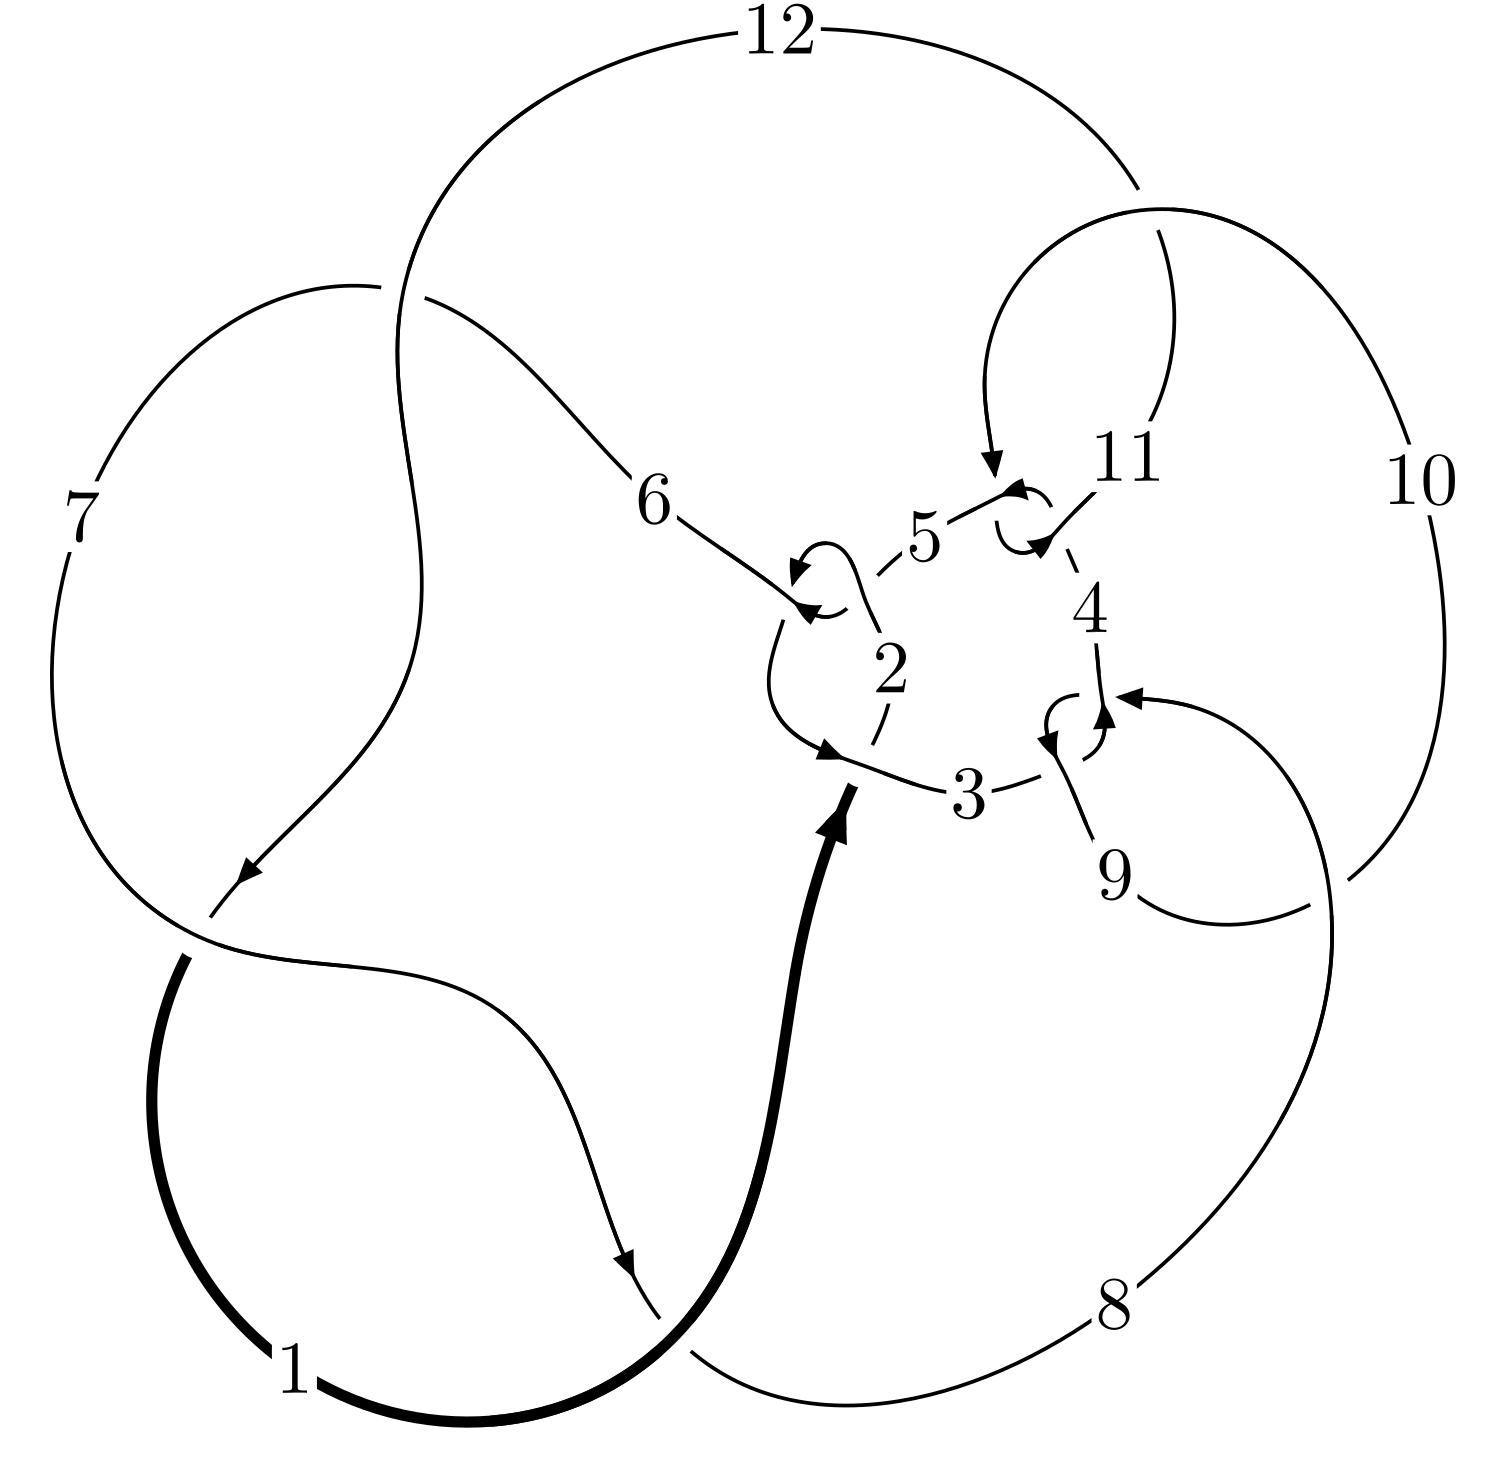
\includegraphics[width=112pt]{../../../GIT/diagram.site/Diagrams/png/1197_12a_0396.png}\\
\ \ \ A knot diagram\footnotemark}&
\allowdisplaybreaks
\textbf{Linearized knot diagam} \\
\cline{2-2}
 &
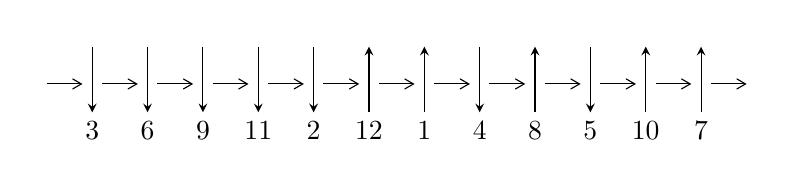
\begin{tikzpicture}[x=20pt, y=17pt]
	% nodes
	\node (C0) at (0, 0) {};
	\node (C1) at (1, 0) {};
	\node (C1U) at (1, +1) {};
	\node (C1D) at (1, -1) {3};

	\node (C2) at (2, 0) {};
	\node (C2U) at (2, +1) {};
	\node (C2D) at (2, -1) {6};

	\node (C3) at (3, 0) {};
	\node (C3U) at (3, +1) {};
	\node (C3D) at (3, -1) {9};

	\node (C4) at (4, 0) {};
	\node (C4U) at (4, +1) {};
	\node (C4D) at (4, -1) {11};

	\node (C5) at (5, 0) {};
	\node (C5U) at (5, +1) {};
	\node (C5D) at (5, -1) {2};

	\node (C6) at (6, 0) {};
	\node (C6U) at (6, +1) {};
	\node (C6D) at (6, -1) {12};

	\node (C7) at (7, 0) {};
	\node (C7U) at (7, +1) {};
	\node (C7D) at (7, -1) {1};

	\node (C8) at (8, 0) {};
	\node (C8U) at (8, +1) {};
	\node (C8D) at (8, -1) {4};

	\node (C9) at (9, 0) {};
	\node (C9U) at (9, +1) {};
	\node (C9D) at (9, -1) {8};

	\node (C10) at (10, 0) {};
	\node (C10U) at (10, +1) {};
	\node (C10D) at (10, -1) {5};

	\node (C11) at (11, 0) {};
	\node (C11U) at (11, +1) {};
	\node (C11D) at (11, -1) {10};

	\node (C12) at (12, 0) {};
	\node (C12U) at (12, +1) {};
	\node (C12D) at (12, -1) {7};
	\node (C13) at (13, 0) {};

	% arrows
	\draw[->,>={angle 60}]
	(C0) edge (C1) (C1) edge (C2) (C2) edge (C3) (C3) edge (C4) (C4) edge (C5) (C5) edge (C6) (C6) edge (C7) (C7) edge (C8) (C8) edge (C9) (C9) edge (C10) (C10) edge (C11) (C11) edge (C12) (C12) edge (C13) ;	\draw[->,>=stealth]
	(C1U) edge (C1D) (C2U) edge (C2D) (C3U) edge (C3D) (C4U) edge (C4D) (C5U) edge (C5D) (C6D) edge (C6U) (C7D) edge (C7U) (C8U) edge (C8D) (C9D) edge (C9U) (C10U) edge (C10D) (C11D) edge (C11U) (C12D) edge (C12U) ;
	\end{tikzpicture} \\
\hhline{~~} \\& 
\textbf{Solving Sequence} \\ \cline{2-2} 
 &
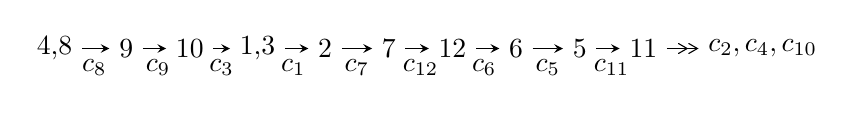
\begin{tikzpicture}[x=23pt, y=7pt]
	% node
	\node (A0) at (-1/8, 0) {4,8};
	\node (A1) at (1, 0) {9};
	\node (A2) at (2, 0) {10};
	\node (A3) at (49/16, 0) {1,3};
	\node (A4) at (33/8, 0) {2};
	\node (A5) at (41/8, 0) {7};
	\node (A6) at (49/8, 0) {12};
	\node (A7) at (57/8, 0) {6};
	\node (A8) at (65/8, 0) {5};
	\node (A9) at (73/8, 0) {11};
	\node (C1) at (1/2, -1) {$c_{8}$};
	\node (C2) at (3/2, -1) {$c_{9}$};
	\node (C3) at (5/2, -1) {$c_{3}$};
	\node (C4) at (29/8, -1) {$c_{1}$};
	\node (C5) at (37/8, -1) {$c_{7}$};
	\node (C6) at (45/8, -1) {$c_{12}$};
	\node (C7) at (53/8, -1) {$c_{6}$};
	\node (C8) at (61/8, -1) {$c_{5}$};
	\node (C9) at (69/8, -1) {$c_{11}$};
	\node (A10) at (11, 0) {$c_{2},c_{4},c_{10}$};

	% edge
	\draw[->,>=stealth]	
	(A0) edge (A1) (A1) edge (A2) (A2) edge (A3) (A3) edge (A4) (A4) edge (A5) (A5) edge (A6) (A6) edge (A7) (A7) edge (A8) (A8) edge (A9) ;
	\draw[->>,>={angle 60}]	
	(A9) edge (A10);
\end{tikzpicture} \\ 

\end{tabular} \\

\footnotetext{
The image of knot diagram is generated by the software ``\textbf{Draw programme}" developed by Andrew Bartholomew(\url{http://www.layer8.co.uk/maths/draw/index.htm\#Running-draw}), where we modified some parts for our purpose(\url{https://github.com/CATsTAILs/LinksPainter}).
}\phantom \\ \newline 
\centering \textbf{Ideals for irreducible components\footnotemark of $X_{\text{par}}$} 
 
\begin{align*}
I^u_{1}&=\langle 
-8 u^{32}-8 u^{31}+\cdots+16 b-30,\;5 u^{32}+9 u^{31}+\cdots+32 a+50,\;u^{33}+7 u^{31}+\cdots+6 u^2+2\rangle \\
I^u_{2}&=\langle 
-2.64825\times10^{24} u^{49}-8.95879\times10^{24} u^{48}+\cdots+5.05220\times10^{25} b-7.19242\times10^{25},\\
\phantom{I^u_{2}}&\phantom{= \langle  }-1.59826\times10^{25} u^{49}-1.45944\times10^{25} u^{48}+\cdots+5.05220\times10^{25} a+1.62536\times10^{26},\\
\phantom{I^u_{2}}&\phantom{= \langle  }u^{50}+2 u^{49}+\cdots+44 u+8\rangle \\
I^u_{3}&=\langle 
- u^3 a+a^2 u-2 u^3- a^2- a u+2 b-2 a-2,\\
\phantom{I^u_{3}}&\phantom{= \langle  }2 u^3 a^2-2 a^2 u^2+u^3 a+2 a^3+4 a^2 u-3 u^2 a+u^3+2 a^2-3 u^2+a+2 u-1,\;u^4+u^2+u+1\rangle \\
I^u_{4}&=\langle 
b-1,\;u^2+2 a+u,\;u^4+u^2+2\rangle \\
I^u_{5}&=\langle 
a^3 u+a^3- a^2 u+2 a^2-3 a u+b-3 a- u-3,\;2 a^4-3 a^3 u+a^3-6 a^2+3 a u-5 a+u-1,\;u^2+1\rangle \\
I^u_{6}&=\langle 
- u^5 a^2+2 u^5 a+\cdots-4 a+4,\\
\phantom{I^u_{6}}&\phantom{= \langle  }2 u^5 a^2-2 u^5 a+2 u^3 a^2+3 u^4 a-2 a^2 u^2-3 u^3 a+2 u^4+a^3+2 a^2 u+2 u^2 a-2 a^2-4 a u+2 u^2+4 a-2 u,\\
\phantom{I^u_{6}}&\phantom{= \langle  }u^6- u^5+2 u^4-2 u^3+2 u^2-2 u+1\rangle \\
I^u_{7}&=\langle 
b+1,\;u^3- u^2+2 a+u+1,\;u^4+1\rangle \\
\\
I^v_{1}&=\langle 
a,\;b+1,\;v-1\rangle \\
\end{align*}
\raggedright * 8 irreducible components of $\dim_{\mathbb{C}}=0$, with total 130 representations.\\
\footnotetext{All coefficients of polynomials are rational numbers. But the coefficients are sometimes approximated in decimal forms when there is not enough margin.}
\newpage
\renewcommand{\arraystretch}{1}
\centering \section*{I. $I^u_{1}= \langle -8 u^{32}-8 u^{31}+\cdots+16 b-30,\;5 u^{32}+9 u^{31}+\cdots+32 a+50,\;u^{33}+7 u^{31}+\cdots+6 u^2+2 \rangle$}
\flushleft \textbf{(i) Arc colorings}\\
\begin{tabular}{m{7pt} m{180pt} m{7pt} m{180pt} }
\flushright $a_{4}=$&$\begin{pmatrix}0\\u\end{pmatrix}$ \\
\flushright $a_{8}=$&$\begin{pmatrix}1\\0\end{pmatrix}$ \\
\flushright $a_{9}=$&$\begin{pmatrix}1\\u^2\end{pmatrix}$ \\
\flushright $a_{10}=$&$\begin{pmatrix}u^2+1\\u^2\end{pmatrix}$ \\
\flushright $a_{1}=$&$\begin{pmatrix}-0.156250 u^{32}-0.281250 u^{31}+\cdots+0.187500 u-1.56250\\\frac{1}{2} u^{32}+\frac{1}{2} u^{31}+\cdots+\frac{21}{8} u+\frac{15}{8}\end{pmatrix}$ \\
\flushright $a_{3}=$&$\begin{pmatrix}u\\u^3+u\end{pmatrix}$ \\
\flushright $a_{2}=$&$\begin{pmatrix}0.156250 u^{32}-0.218750 u^{31}+\cdots+1.43750 u-0.562500\\0.687500 u^{32}+0.687500 u^{31}+\cdots+3.25000 u+2.75000\end{pmatrix}$ \\
\flushright $a_{7}=$&$\begin{pmatrix}0.281250 u^{32}+0.281250 u^{31}+\cdots+0.812500 u+1.56250\\\frac{3}{16} u^{32}-\frac{9}{16} u^{31}+\cdots+\frac{9}{8} u-\frac{11}{8}\end{pmatrix}$ \\
\flushright $a_{12}=$&$\begin{pmatrix}- u^4- u^2-1\\-\frac{1}{8} u^{31}-\frac{3}{4} u^{29}+\cdots-\frac{5}{2} u^2-\frac{1}{4}\end{pmatrix}$ \\
\flushright $a_{6}=$&$\begin{pmatrix}-0.156250 u^{32}+0.218750 u^{31}+\cdots-1.43750 u+0.562500\\\frac{1}{4} u^{32}+\frac{3}{16} u^{31}+\cdots+\frac{25}{8} u+\frac{5}{4}\end{pmatrix}$ \\
\flushright $a_{5}=$&$\begin{pmatrix}- u\\-\frac{1}{8} u^{32}-\frac{3}{4} u^{30}+\cdots-\frac{5}{2} u^3+\frac{3}{4} u\end{pmatrix}$ \\
\flushright $a_{11}=$&$\begin{pmatrix}-1\\-\frac{1}{8} u^{31}-\frac{3}{4} u^{29}+\cdots-\frac{5}{2} u^2-\frac{1}{4}\end{pmatrix}$\\&\end{tabular}
\flushleft \textbf{(ii) Obstruction class $= -1$}\\~\\
\flushleft \textbf{(iii) Cusp Shapes $= -\frac{23}{8} u^{32}+\frac{11}{8} u^{31}+\cdots-\frac{29}{4} u+\frac{17}{4}$}\\~\\
\newpage\renewcommand{\arraystretch}{1}
\flushleft \textbf{(iv) u-Polynomials at the component}\newline \\
\begin{tabular}{m{50pt}|m{274pt}}
Crossings & \hspace{64pt}u-Polynomials at each crossing \\
\hline $$\begin{aligned}c_{1}\end{aligned}$$&$\begin{aligned}
&u^{33}+12 u^{32}+\cdots+521 u+121
\end{aligned}$\\
\hline $$\begin{aligned}c_{2},c_{5}\end{aligned}$$&$\begin{aligned}
&u^{33}+6 u^{32}+\cdots+31 u+11
\end{aligned}$\\
\hline $$\begin{aligned}c_{3},c_{4},c_{8}\\c_{10}\end{aligned}$$&$\begin{aligned}
&u^{33}+7 u^{31}+\cdots+6 u^2+2
\end{aligned}$\\
\hline $$\begin{aligned}c_{6},c_{7},c_{12}\end{aligned}$$&$\begin{aligned}
&u^{33}-6 u^{32}+\cdots+43 u+11
\end{aligned}$\\
\hline $$\begin{aligned}c_{9},c_{11}\end{aligned}$$&$\begin{aligned}
&u^{33}-14 u^{32}+\cdots-24 u+4
\end{aligned}$\\
\hline
\end{tabular}\\~\\
\newpage\renewcommand{\arraystretch}{1}
\flushleft \textbf{(v) Riley Polynomials at the component}\newline \\
\begin{tabular}{m{50pt}|m{274pt}}
Crossings & \hspace{64pt}Riley Polynomials at each crossing \\
\hline $$\begin{aligned}c_{1}\end{aligned}$$&$\begin{aligned}
&y^{33}+24 y^{32}+\cdots-121083 y-14641
\end{aligned}$\\
\hline $$\begin{aligned}c_{2},c_{5}\end{aligned}$$&$\begin{aligned}
&y^{33}-12 y^{32}+\cdots+521 y-121
\end{aligned}$\\
\hline $$\begin{aligned}c_{3},c_{4},c_{8}\\c_{10}\end{aligned}$$&$\begin{aligned}
&y^{33}+14 y^{32}+\cdots-24 y-4
\end{aligned}$\\
\hline $$\begin{aligned}c_{6},c_{7},c_{12}\end{aligned}$$&$\begin{aligned}
&y^{33}-36 y^{32}+\cdots+441 y-121
\end{aligned}$\\
\hline $$\begin{aligned}c_{9},c_{11}\end{aligned}$$&$\begin{aligned}
&y^{33}+18 y^{32}+\cdots+1024 y-16
\end{aligned}$\\
\hline
\end{tabular}\\~\\
\newpage\flushleft \textbf{(vi) Complex Volumes and Cusp Shapes}
$$\begin{array}{c|c|c}  
\text{Solutions to }I^u_{1}& \I (\text{vol} + \sqrt{-1}CS) & \text{Cusp shape}\\
 \hline 
\begin{aligned}
u &= -0.915077 + 0.392052 I \\
a &= \phantom{-}0.964198 - 0.704112 I \\
b &= \phantom{-}1.39433 - 0.29710 I\end{aligned}
 & \phantom{-}1.39980 - 6.40207 I & -2.78525 + 3.47464 I \\ \hline\begin{aligned}
u &= -0.915077 - 0.392052 I \\
a &= \phantom{-}0.964198 + 0.704112 I \\
b &= \phantom{-}1.39433 + 0.29710 I\end{aligned}
 & \phantom{-}1.39980 + 6.40207 I & -2.78525 - 3.47464 I \\ \hline\begin{aligned}
u &= \phantom{-}0.521343 + 0.878780 I \\
a &= \phantom{-}0.278469 + 1.164920 I \\
b &= -1.006190 + 0.409437 I\end{aligned}
 & \phantom{-}1.86625 - 5.18521 I & \phantom{-}2.35796 + 8.34892 I \\ \hline\begin{aligned}
u &= \phantom{-}0.521343 - 0.878780 I \\
a &= \phantom{-}0.278469 - 1.164920 I \\
b &= -1.006190 - 0.409437 I\end{aligned}
 & \phantom{-}1.86625 + 5.18521 I & \phantom{-}2.35796 - 8.34892 I \\ \hline\begin{aligned}
u &= \phantom{-}0.717553 + 0.749593 I \\
a &= \phantom{-}0.129136 - 1.144270 I \\
b &= \phantom{-}0.033872 - 0.657961 I\end{aligned}
 & -4.49859 - 4.89069 I & -7.87872 + 6.56643 I \\ \hline\begin{aligned}
u &= \phantom{-}0.717553 - 0.749593 I \\
a &= \phantom{-}0.129136 + 1.144270 I \\
b &= \phantom{-}0.033872 + 0.657961 I\end{aligned}
 & -4.49859 + 4.89069 I & -7.87872 - 6.56643 I \\ \hline\begin{aligned}
u &= \phantom{-}0.347167 + 1.041210 I \\
a &= -0.857157 - 0.206509 I \\
b &= \phantom{-}1.59638 + 0.20692 I\end{aligned}
 & \phantom{-}10.63600 + 1.24046 I & \phantom{-}4.58607 + 3.80858 I \\ \hline\begin{aligned}
u &= \phantom{-}0.347167 - 1.041210 I \\
a &= -0.857157 + 0.206509 I \\
b &= \phantom{-}1.59638 - 0.20692 I\end{aligned}
 & \phantom{-}10.63600 - 1.24046 I & \phantom{-}4.58607 - 3.80858 I \\ \hline\begin{aligned}
u &= \phantom{-}0.762745 + 0.444328 I \\
a &= -0.56231 - 1.38622 I \\
b &= -0.196556 - 0.752591 I\end{aligned}
 & -3.68416 + 2.61049 I & -7.80738 - 1.77247 I \\ \hline\begin{aligned}
u &= \phantom{-}0.762745 - 0.444328 I \\
a &= -0.56231 + 1.38622 I \\
b &= -0.196556 + 0.752591 I\end{aligned}
 & -3.68416 - 2.61049 I & -7.80738 + 1.77247 I\\
 \hline 
 \end{array}$$\newpage$$\begin{array}{c|c|c}  
\text{Solutions to }I^u_{1}& \I (\text{vol} + \sqrt{-1}CS) & \text{Cusp shape}\\
 \hline 
\begin{aligned}
u &= \phantom{-}0.823813 + 0.245550 I \\
a &= \phantom{-}0.805044 + 0.420154 I \\
b &= \phantom{-}1.365110 + 0.173472 I\end{aligned}
 & \phantom{-}3.45677 + 1.23306 I & -0.418871 + 0.738062 I \\ \hline\begin{aligned}
u &= \phantom{-}0.823813 - 0.245550 I \\
a &= \phantom{-}0.805044 - 0.420154 I \\
b &= \phantom{-}1.365110 - 0.173472 I\end{aligned}
 & \phantom{-}3.45677 - 1.23306 I & -0.418871 - 0.738062 I \\ \hline\begin{aligned}
u &= -0.473645 + 1.050870 I \\
a &= -0.268275 + 0.246204 I \\
b &= -0.657658 + 0.770559 I\end{aligned}
 & \phantom{-}3.04967 + 2.32264 I & \phantom{-}1.80922 - 1.99961 I \\ \hline\begin{aligned}
u &= -0.473645 - 1.050870 I \\
a &= -0.268275 - 0.246204 I \\
b &= -0.657658 - 0.770559 I\end{aligned}
 & \phantom{-}3.04967 - 2.32264 I & \phantom{-}1.80922 + 1.99961 I \\ \hline\begin{aligned}
u &= -0.396598 + 1.108560 I \\
a &= -0.883813 + 0.566525 I \\
b &= \phantom{-}1.61157 - 0.05524 I\end{aligned}
 & \phantom{-}11.59150 + 5.51497 I & \phantom{-}5.96018 - 7.21704 I \\ \hline\begin{aligned}
u &= -0.396598 - 1.108560 I \\
a &= -0.883813 - 0.566525 I \\
b &= \phantom{-}1.61157 + 0.05524 I\end{aligned}
 & \phantom{-}11.59150 - 5.51497 I & \phantom{-}5.96018 + 7.21704 I \\ \hline\begin{aligned}
u &= -0.835942 + 0.860558 I \\
a &= -0.692058 - 1.146520 I \\
b &= -1.296420 - 0.210819 I\end{aligned}
 & -0.38293 + 7.96970 I & -0.94048 - 8.93222 I \\ \hline\begin{aligned}
u &= -0.835942 - 0.860558 I \\
a &= -0.692058 + 1.146520 I \\
b &= -1.296420 + 0.210819 I\end{aligned}
 & -0.38293 - 7.96970 I & -0.94048 + 8.93222 I \\ \hline\begin{aligned}
u &= -0.649902 + 1.037910 I \\
a &= \phantom{-}0.858076 - 0.606711 I \\
b &= -0.185341 - 0.364626 I\end{aligned}
 & -2.69171 + 5.74108 I & -6.75405 - 5.32867 I \\ \hline\begin{aligned}
u &= -0.649902 - 1.037910 I \\
a &= \phantom{-}0.858076 + 0.606711 I \\
b &= -0.185341 + 0.364626 I\end{aligned}
 & -2.69171 - 5.74108 I & -6.75405 + 5.32867 I\\
 \hline 
 \end{array}$$\newpage$$\begin{array}{c|c|c}  
\text{Solutions to }I^u_{1}& \I (\text{vol} + \sqrt{-1}CS) & \text{Cusp shape}\\
 \hline 
\begin{aligned}
u &= \phantom{-}0.040993 + 0.770747 I \\
a &= \phantom{-}1.47224 + 0.23255 I \\
b &= -1.59948 + 0.10021 I\end{aligned}
 & \phantom{-}9.08975 - 3.34368 I & -2.92320 + 4.06886 I \\ \hline\begin{aligned}
u &= \phantom{-}0.040993 - 0.770747 I \\
a &= \phantom{-}1.47224 - 0.23255 I \\
b &= -1.59948 - 0.10021 I\end{aligned}
 & \phantom{-}9.08975 + 3.34368 I & -2.92320 - 4.06886 I \\ \hline\begin{aligned}
u &= \phantom{-}0.771934 + 1.013930 I \\
a &= -0.632971 + 0.675979 I \\
b &= -1.245670 - 0.061329 I\end{aligned}
 & \phantom{-}0.57566 - 4.29905 I & \phantom{-}2.61702 + 1.07304 I \\ \hline\begin{aligned}
u &= \phantom{-}0.771934 - 1.013930 I \\
a &= -0.632971 - 0.675979 I \\
b &= -1.245670 + 0.061329 I\end{aligned}
 & \phantom{-}0.57566 + 4.29905 I & \phantom{-}2.61702 - 1.07304 I \\ \hline\begin{aligned}
u &= -0.591756 + 1.172490 I \\
a &= \phantom{-}0.718848 - 1.111970 I \\
b &= -0.333529 - 0.923419 I\end{aligned}
 & \phantom{-}0.84237 + 13.11040 I & -0.78548 - 9.94308 I \\ \hline\begin{aligned}
u &= -0.591756 - 1.172490 I \\
a &= \phantom{-}0.718848 + 1.111970 I \\
b &= -0.333529 + 0.923419 I\end{aligned}
 & \phantom{-}0.84237 - 13.11040 I & -0.78548 + 9.94308 I \\ \hline\begin{aligned}
u &= -0.564519 + 1.207290 I \\
a &= -0.64338 + 1.66167 I \\
b &= \phantom{-}1.51399 + 0.28516 I\end{aligned}
 & \phantom{-}9.1548 + 11.5989 I & \phantom{-}4.91327 - 6.70032 I \\ \hline\begin{aligned}
u &= -0.564519 - 1.207290 I \\
a &= -0.64338 - 1.66167 I \\
b &= \phantom{-}1.51399 - 0.28516 I\end{aligned}
 & \phantom{-}9.1548 - 11.5989 I & \phantom{-}4.91327 + 6.70032 I \\ \hline\begin{aligned}
u &= \phantom{-}0.609861 + 1.220400 I \\
a &= -0.47129 - 1.90074 I \\
b &= \phantom{-}1.47614 - 0.36873 I\end{aligned}
 & \phantom{-}6.6338 - 17.7809 I & \phantom{-}2.21241 + 10.23989 I \\ \hline\begin{aligned}
u &= \phantom{-}0.609861 - 1.220400 I \\
a &= -0.47129 + 1.90074 I \\
b &= \phantom{-}1.47614 + 0.36873 I\end{aligned}
 & \phantom{-}6.6338 + 17.7809 I & \phantom{-}2.21241 - 10.23989 I\\
 \hline 
 \end{array}$$\newpage$$\begin{array}{c|c|c}  
\text{Solutions to }I^u_{1}& \I (\text{vol} + \sqrt{-1}CS) & \text{Cusp shape}\\
 \hline 
\begin{aligned}
u &= \phantom{-}0.028409 + 0.547371 I \\
a &= -0.373780 + 0.278891 I \\
b &= \phantom{-}0.692239 + 0.437691 I\end{aligned}
 & \phantom{-}1.18727 + 1.45039 I & \phantom{-}0.42798 - 3.86280 I \\ \hline\begin{aligned}
u &= \phantom{-}0.028409 - 0.547371 I \\
a &= -0.373780 - 0.278891 I \\
b &= \phantom{-}0.692239 - 0.437691 I\end{aligned}
 & \phantom{-}1.18727 - 1.45039 I & \phantom{-}0.42798 + 3.86280 I \\ \hline\begin{aligned}
u &= -0.392754\phantom{ +0.000000I} \\
a &= -1.68195\phantom{ +0.000000I} \\
b &= -0.325593\phantom{ +0.000000I}\end{aligned}
 & -1.04636\phantom{ +0.000000I} & -11.1810\phantom{ +0.000000I}\\
 \hline 
 \end{array}$$\newpage\newpage\renewcommand{\arraystretch}{1}
\centering \section*{II. $I^u_{2}= \langle -2.65\times10^{24} u^{49}-8.96\times10^{24} u^{48}+\cdots+5.05\times10^{25} b-7.19\times10^{25},\;-1.60\times10^{25} u^{49}-1.46\times10^{25} u^{48}+\cdots+5.05\times10^{25} a+1.63\times10^{26},\;u^{50}+2 u^{49}+\cdots+44 u+8 \rangle$}
\flushleft \textbf{(i) Arc colorings}\\
\begin{tabular}{m{7pt} m{180pt} m{7pt} m{180pt} }
\flushright $a_{4}=$&$\begin{pmatrix}0\\u\end{pmatrix}$ \\
\flushright $a_{8}=$&$\begin{pmatrix}1\\0\end{pmatrix}$ \\
\flushright $a_{9}=$&$\begin{pmatrix}1\\u^2\end{pmatrix}$ \\
\flushright $a_{10}=$&$\begin{pmatrix}u^2+1\\u^2\end{pmatrix}$ \\
\flushright $a_{1}=$&$\begin{pmatrix}0.316348 u^{49}+0.288873 u^{48}+\cdots-5.69866 u-3.21712\\0.0524177 u^{49}+0.177324 u^{48}+\cdots+6.15670 u+1.42362\end{pmatrix}$ \\
\flushright $a_{3}=$&$\begin{pmatrix}u\\u^3+u\end{pmatrix}$ \\
\flushright $a_{2}=$&$\begin{pmatrix}0.331848 u^{49}+0.381211 u^{48}+\cdots+2.15589 u-1.40233\\0.0642354 u^{49}+0.233571 u^{48}+\cdots+11.1884 u+2.74771\end{pmatrix}$ \\
\flushright $a_{7}=$&$\begin{pmatrix}0.396469 u^{49}+0.617854 u^{48}+\cdots+9.00772 u+1.32807\\0.270674 u^{49}+0.480833 u^{48}+\cdots+15.1832 u+3.08494\end{pmatrix}$ \\
\flushright $a_{12}=$&$\begin{pmatrix}0.355248 u^{49}+0.291595 u^{48}+\cdots-0.394990 u-1.10912\\0.0482855 u^{49}+0.111160 u^{48}+\cdots+5.80109 u+2.01284\end{pmatrix}$ \\
\flushright $a_{6}=$&$\begin{pmatrix}0.421552 u^{49}+0.618093 u^{48}+\cdots+0.335698 u-2.40068\\0.261028 u^{49}+0.573430 u^{48}+\cdots+19.0608 u+4.00464\end{pmatrix}$ \\
\flushright $a_{5}=$&$\begin{pmatrix}0.181884 u^{49}+0.334958 u^{48}+\cdots-4.80912 u-2.81382\\0.306884 u^{49}+0.584958 u^{48}+\cdots+16.4409 u+2.68618\end{pmatrix}$ \\
\flushright $a_{11}=$&$\begin{pmatrix}0.335773 u^{49}+0.364661 u^{48}+\cdots+4.62064 u-0.666888\\1\end{pmatrix}$\\&\end{tabular}
\flushleft \textbf{(ii) Obstruction class $= -1$}\\~\\
\flushleft \textbf{(iii) Cusp Shapes $= -\frac{1898522637621677506109549}{3157627707198910369381082} u^{49}-\frac{4020305257773637481583771}{6315255414397820738762164} u^{48}+\cdots-\frac{11335271725021575919299381}{1578813853599455184690541} u+\frac{1203508006065254918095845}{1578813853599455184690541}$}\\~\\
\newpage\renewcommand{\arraystretch}{1}
\flushleft \textbf{(iv) u-Polynomials at the component}\newline \\
\begin{tabular}{m{50pt}|m{274pt}}
Crossings & \hspace{64pt}u-Polynomials at each crossing \\
\hline $$\begin{aligned}c_{1}\end{aligned}$$&$\begin{aligned}
&(u^{25}+10 u^{24}+\cdots+97 u+9)^{2}
\end{aligned}$\\
\hline $$\begin{aligned}c_{2},c_{5}\end{aligned}$$&$\begin{aligned}
&(u^{25}-2 u^{24}+\cdots- u+3)^{2}
\end{aligned}$\\
\hline $$\begin{aligned}c_{3},c_{4},c_{8}\\c_{10}\end{aligned}$$&$\begin{aligned}
&u^{50}+2 u^{49}+\cdots+44 u+8
\end{aligned}$\\
\hline $$\begin{aligned}c_{6},c_{7},c_{12}\end{aligned}$$&$\begin{aligned}
&(u^{25}+2 u^{24}+\cdots-5 u+3)^{2}
\end{aligned}$\\
\hline $$\begin{aligned}c_{9},c_{11}\end{aligned}$$&$\begin{aligned}
&u^{50}-28 u^{49}+\cdots-784 u+64
\end{aligned}$\\
\hline
\end{tabular}\\~\\
\newpage\renewcommand{\arraystretch}{1}
\flushleft \textbf{(v) Riley Polynomials at the component}\newline \\
\begin{tabular}{m{50pt}|m{274pt}}
Crossings & \hspace{64pt}Riley Polynomials at each crossing \\
\hline $$\begin{aligned}c_{1}\end{aligned}$$&$\begin{aligned}
&(y^{25}+14 y^{24}+\cdots+1561 y-81)^{2}
\end{aligned}$\\
\hline $$\begin{aligned}c_{2},c_{5}\end{aligned}$$&$\begin{aligned}
&(y^{25}-10 y^{24}+\cdots+97 y-9)^{2}
\end{aligned}$\\
\hline $$\begin{aligned}c_{3},c_{4},c_{8}\\c_{10}\end{aligned}$$&$\begin{aligned}
&y^{50}+28 y^{49}+\cdots+784 y+64
\end{aligned}$\\
\hline $$\begin{aligned}c_{6},c_{7},c_{12}\end{aligned}$$&$\begin{aligned}
&(y^{25}-26 y^{24}+\cdots-47 y-9)^{2}
\end{aligned}$\\
\hline $$\begin{aligned}c_{9},c_{11}\end{aligned}$$&$\begin{aligned}
&y^{50}-12 y^{49}+\cdots+68864 y+4096
\end{aligned}$\\
\hline
\end{tabular}\\~\\
\newpage\flushleft \textbf{(vi) Complex Volumes and Cusp Shapes}
$$\begin{array}{c|c|c}  
\text{Solutions to }I^u_{2}& \I (\text{vol} + \sqrt{-1}CS) & \text{Cusp shape}\\
 \hline 
\begin{aligned}
u &= \phantom{-}0.966918 + 0.270016 I \\
a &= -0.751464 - 0.895075 I \\
b &= -1.44066 - 0.34360 I\end{aligned}
 & \phantom{-}3.73131 + 12.07650 I & -0.57661 - 7.22441 I \\ \hline\begin{aligned}
u &= \phantom{-}0.966918 - 0.270016 I \\
a &= -0.751464 + 0.895075 I \\
b &= -1.44066 + 0.34360 I\end{aligned}
 & \phantom{-}3.73131 - 12.07650 I & -0.57661 + 7.22441 I \\ \hline\begin{aligned}
u &= -0.775444 + 0.545505 I \\
a &= -0.414542 - 0.876936 I \\
b &= \phantom{-}0.066602 - 0.499012 I\end{aligned}
 & -4.14430 - 0.37131 I & -8.72924 - 0.01538 I \\ \hline\begin{aligned}
u &= -0.775444 - 0.545505 I \\
a &= -0.414542 + 0.876936 I \\
b &= \phantom{-}0.066602 + 0.499012 I\end{aligned}
 & -4.14430 + 0.37131 I & -8.72924 + 0.01538 I \\ \hline\begin{aligned}
u &= \phantom{-}0.201989 + 1.059430 I \\
a &= -0.09976 + 1.59657 I \\
b &= -0.708151\phantom{ +0.000000I}\end{aligned}
 & \phantom{-}4.19892\phantom{ +0.000000I} & \phantom{-}8.09367 + 0. I\phantom{ +0.000000I} \\ \hline\begin{aligned}
u &= \phantom{-}0.201989 - 1.059430 I \\
a &= -0.09976 - 1.59657 I \\
b &= -0.708151\phantom{ +0.000000I}\end{aligned}
 & \phantom{-}4.19892\phantom{ +0.000000I} & \phantom{-}8.09367 + 0. I\phantom{ +0.000000I} \\ \hline\begin{aligned}
u &= -0.869538 + 0.298974 I \\
a &= \phantom{-}0.334522 - 1.368370 I \\
b &= \phantom{-}0.281632 - 0.858743 I\end{aligned}
 & -1.77513 - 7.73599 I & -4.26723 + 6.67404 I \\ \hline\begin{aligned}
u &= -0.869538 - 0.298974 I \\
a &= \phantom{-}0.334522 + 1.368370 I \\
b &= \phantom{-}0.281632 + 0.858743 I\end{aligned}
 & -1.77513 + 7.73599 I & -4.26723 - 6.67404 I \\ \hline\begin{aligned}
u &= -0.895045 + 0.202572 I \\
a &= -0.593420 + 0.550719 I \\
b &= -1.45092 + 0.25712 I\end{aligned}
 & \phantom{-}6.14042 - 6.29490 I & \phantom{-}2.20266 + 3.49250 I \\ \hline\begin{aligned}
u &= -0.895045 - 0.202572 I \\
a &= -0.593420 - 0.550719 I \\
b &= -1.45092 - 0.25712 I\end{aligned}
 & \phantom{-}6.14042 + 6.29490 I & \phantom{-}2.20266 - 3.49250 I\\
 \hline 
 \end{array}$$\newpage$$\begin{array}{c|c|c}  
\text{Solutions to }I^u_{2}& \I (\text{vol} + \sqrt{-1}CS) & \text{Cusp shape}\\
 \hline 
\begin{aligned}
u &= \phantom{-}0.665448 + 0.869585 I \\
a &= -0.918930 - 0.862702 I \\
b &= \phantom{-}0.066602 - 0.499012 I\end{aligned}
 & -4.14430 - 0.37131 I & -8.72924 + 0. I\phantom{ +0.000000I} \\ \hline\begin{aligned}
u &= \phantom{-}0.665448 - 0.869585 I \\
a &= -0.918930 + 0.862702 I \\
b &= \phantom{-}0.066602 + 0.499012 I\end{aligned}
 & -4.14430 + 0.37131 I & -8.72924 + 0. I\phantom{ +0.000000I} \\ \hline\begin{aligned}
u &= -0.437535 + 1.037370 I \\
a &= \phantom{-}0.79029 - 1.70199 I \\
b &= -0.360930 - 0.736826 I\end{aligned}
 & \phantom{-}3.32486 + 4.24383 I & \phantom{-}0.60496 - 6.78537 I \\ \hline\begin{aligned}
u &= -0.437535 - 1.037370 I \\
a &= \phantom{-}0.79029 + 1.70199 I \\
b &= -0.360930 + 0.736826 I\end{aligned}
 & \phantom{-}3.32486 - 4.24383 I & \phantom{-}0.60496 + 6.78537 I \\ \hline\begin{aligned}
u &= \phantom{-}0.898759 + 0.681190 I \\
a &= \phantom{-}0.898999 - 0.731480 I \\
b &= \phantom{-}1.273790 - 0.131362 I\end{aligned}
 & -0.43185 - 1.83282 I & \phantom{-0.000000 -}0. + 4.01286 I \\ \hline\begin{aligned}
u &= \phantom{-}0.898759 - 0.681190 I \\
a &= \phantom{-}0.898999 + 0.731480 I \\
b &= \phantom{-}1.273790 + 0.131362 I\end{aligned}
 & -0.43185 + 1.83282 I & \phantom{-0.000000 } 0. - 4.01286 I \\ \hline\begin{aligned}
u &= -0.024231 + 1.181170 I \\
a &= \phantom{-}0.523985 + 0.397590 I \\
b &= \phantom{-}0.276341 + 0.419444 I\end{aligned}
 & \phantom{-}1.76402 + 1.04428 I & -5.27127 - 1.42914 I \\ \hline\begin{aligned}
u &= -0.024231 - 1.181170 I \\
a &= \phantom{-}0.523985 - 0.397590 I \\
b &= \phantom{-}0.276341 - 0.419444 I\end{aligned}
 & \phantom{-}1.76402 - 1.04428 I & -5.27127 + 1.42914 I \\ \hline\begin{aligned}
u &= -0.836400 + 0.845826 I \\
a &= \phantom{-}0.914347 + 0.357065 I \\
b &= \phantom{-}1.273790 - 0.131362 I\end{aligned}
 & -0.43185 - 1.83282 I & \phantom{-0.000000 -}0. + 4.01286 I \\ \hline\begin{aligned}
u &= -0.836400 - 0.845826 I \\
a &= \phantom{-}0.914347 - 0.357065 I \\
b &= \phantom{-}1.273790 + 0.131362 I\end{aligned}
 & -0.43185 + 1.83282 I & \phantom{-0.000000 } 0. - 4.01286 I\\
 \hline 
 \end{array}$$\newpage$$\begin{array}{c|c|c}  
\text{Solutions to }I^u_{2}& \I (\text{vol} + \sqrt{-1}CS) & \text{Cusp shape}\\
 \hline 
\begin{aligned}
u &= \phantom{-}0.550448 + 1.066430 I \\
a &= \phantom{-}0.12223 - 2.40447 I \\
b &= \phantom{-}1.45602 - 0.27617 I\end{aligned}
 & \phantom{-}9.17748 - 7.92352 I & \phantom{-}3.71863 + 6.25521 I \\ \hline\begin{aligned}
u &= \phantom{-}0.550448 - 1.066430 I \\
a &= \phantom{-}0.12223 + 2.40447 I \\
b &= \phantom{-}1.45602 + 0.27617 I\end{aligned}
 & \phantom{-}9.17748 + 7.92352 I & \phantom{-}3.71863 - 6.25521 I \\ \hline\begin{aligned}
u &= \phantom{-}0.209739 + 0.755305 I \\
a &= \phantom{-}0.064242 + 0.285254 I \\
b &= \phantom{-}0.684260 + 0.499844 I\end{aligned}
 & \phantom{-}1.19934 + 1.42730 I & -0.30682 - 4.01748 I \\ \hline\begin{aligned}
u &= \phantom{-}0.209739 - 0.755305 I \\
a &= \phantom{-}0.064242 - 0.285254 I \\
b &= \phantom{-}0.684260 - 0.499844 I\end{aligned}
 & \phantom{-}1.19934 - 1.42730 I & -0.30682 + 4.01748 I \\ \hline\begin{aligned}
u &= -0.486500 + 1.134090 I \\
a &= -0.31834 + 2.07821 I \\
b &= \phantom{-}1.46767 + 0.15865 I\end{aligned}
 & \phantom{-}10.93610 + 2.15851 I & \phantom{-}6.42476 + 0. I\phantom{ +0.000000I} \\ \hline\begin{aligned}
u &= -0.486500 - 1.134090 I \\
a &= -0.31834 - 2.07821 I \\
b &= \phantom{-}1.46767 - 0.15865 I\end{aligned}
 & \phantom{-}10.93610 - 2.15851 I & \phantom{-}6.42476 + 0. I\phantom{ +0.000000I} \\ \hline\begin{aligned}
u &= \phantom{-}0.592659 + 1.085410 I \\
a &= -0.592610 - 1.250100 I \\
b &= \phantom{-}0.281632 - 0.858743 I\end{aligned}
 & -1.77513 - 7.73599 I & \phantom{-0.000000 -}0. + 6.67404 I \\ \hline\begin{aligned}
u &= \phantom{-}0.592659 - 1.085410 I \\
a &= -0.592610 + 1.250100 I \\
b &= \phantom{-}0.281632 + 0.858743 I\end{aligned}
 & -1.77513 + 7.73599 I & \phantom{-0.000000 } 0. - 6.67404 I \\ \hline\begin{aligned}
u &= \phantom{-}0.598799 + 0.472548 I \\
a &= -2.08191 - 0.65289 I \\
b &= -1.43420 - 0.17935 I\end{aligned}
 & \phantom{-}7.40691 + 3.30443 I & \phantom{-}2.15585 - 1.80924 I \\ \hline\begin{aligned}
u &= \phantom{-}0.598799 - 0.472548 I \\
a &= -2.08191 + 0.65289 I \\
b &= -1.43420 + 0.17935 I\end{aligned}
 & \phantom{-}7.40691 - 3.30443 I & \phantom{-}2.15585 + 1.80924 I\\
 \hline 
 \end{array}$$\newpage$$\begin{array}{c|c|c}  
\text{Solutions to }I^u_{2}& \I (\text{vol} + \sqrt{-1}CS) & \text{Cusp shape}\\
 \hline 
\begin{aligned}
u &= \phantom{-}0.230191 + 1.233540 I \\
a &= \phantom{-}0.816301 + 0.437714 I \\
b &= -1.46552 - 0.03322 I\end{aligned}
 & \phantom{-}8.27446 - 2.21818 I & \phantom{-0.000000 } 0 \\ \hline\begin{aligned}
u &= \phantom{-}0.230191 - 1.233540 I \\
a &= \phantom{-}0.816301 - 0.437714 I \\
b &= -1.46552 + 0.03322 I\end{aligned}
 & \phantom{-}8.27446 + 2.21818 I & \phantom{-0.000000 } 0 \\ \hline\begin{aligned}
u &= -0.241098 + 1.258930 I \\
a &= -0.356897 + 0.269220 I \\
b &= -0.360930 + 0.736826 I\end{aligned}
 & \phantom{-}3.32486 - 4.24383 I & \phantom{-0.000000 } 0 \\ \hline\begin{aligned}
u &= -0.241098 - 1.258930 I \\
a &= -0.356897 - 0.269220 I \\
b &= -0.360930 - 0.736826 I\end{aligned}
 & \phantom{-}3.32486 + 4.24383 I & \phantom{-0.000000 } 0 \\ \hline\begin{aligned}
u &= -0.221133 + 0.682614 I \\
a &= \phantom{-}2.02855 - 1.71297 I \\
b &= \phantom{-}0.276341 - 0.419444 I\end{aligned}
 & \phantom{-}1.76402 - 1.04428 I & -5.27127 + 1.42914 I \\ \hline\begin{aligned}
u &= -0.221133 - 0.682614 I \\
a &= \phantom{-}2.02855 + 1.71297 I \\
b &= \phantom{-}0.276341 + 0.419444 I\end{aligned}
 & \phantom{-}1.76402 + 1.04428 I & -5.27127 - 1.42914 I \\ \hline\begin{aligned}
u &= \phantom{-}0.555645 + 1.156390 I \\
a &= \phantom{-}0.45124 + 1.69756 I \\
b &= -1.45092 + 0.25712 I\end{aligned}
 & \phantom{-}6.14042 - 6.29490 I & \phantom{-0.000000 } 0 \\ \hline\begin{aligned}
u &= \phantom{-}0.555645 - 1.156390 I \\
a &= \phantom{-}0.45124 - 1.69756 I \\
b &= -1.45092 - 0.25712 I\end{aligned}
 & \phantom{-}6.14042 + 6.29490 I & \phantom{-0.000000 } 0 \\ \hline\begin{aligned}
u &= -0.100716 + 1.304410 I \\
a &= \phantom{-}0.719569 + 0.115161 I \\
b &= -1.43420 + 0.17935 I\end{aligned}
 & \phantom{-}7.40691 - 3.30443 I & \phantom{-0.000000 } 0 \\ \hline\begin{aligned}
u &= -0.100716 - 1.304410 I \\
a &= \phantom{-}0.719569 - 0.115161 I \\
b &= -1.43420 - 0.17935 I\end{aligned}
 & \phantom{-}7.40691 + 3.30443 I & \phantom{-0.000000 } 0\\
 \hline 
 \end{array}$$\newpage$$\begin{array}{c|c|c}  
\text{Solutions to }I^u_{2}& \I (\text{vol} + \sqrt{-1}CS) & \text{Cusp shape}\\
 \hline 
\begin{aligned}
u &= -0.635007 + 1.157080 I \\
a &= \phantom{-}0.20430 - 1.91387 I \\
b &= -1.44066 - 0.34360 I\end{aligned}
 & \phantom{-}3.73131 + 12.07650 I & \phantom{-0.000000 } 0 \\ \hline\begin{aligned}
u &= -0.635007 - 1.157080 I \\
a &= \phantom{-}0.20430 + 1.91387 I \\
b &= -1.44066 + 0.34360 I\end{aligned}
 & \phantom{-}3.73131 - 12.07650 I & \phantom{-0.000000 } 0 \\ \hline\begin{aligned}
u &= -0.634382 + 0.206664 I \\
a &= -1.45945 + 0.94937 I \\
b &= -1.46552 + 0.03322 I\end{aligned}
 & \phantom{-}8.27446 + 2.21818 I & \phantom{-}3.23817 - 3.39990 I \\ \hline\begin{aligned}
u &= -0.634382 - 0.206664 I \\
a &= -1.45945 - 0.94937 I \\
b &= -1.46552 - 0.03322 I\end{aligned}
 & \phantom{-}8.27446 - 2.21818 I & \phantom{-}3.23817 + 3.39990 I \\ \hline\begin{aligned}
u &= -0.323168 + 1.297610 I \\
a &= -0.805615 + 0.515870 I \\
b &= \phantom{-}1.46767 - 0.15865 I\end{aligned}
 & \phantom{-}10.93610 - 2.15851 I & \phantom{-0.000000 } 0 \\ \hline\begin{aligned}
u &= -0.323168 - 1.297610 I \\
a &= -0.805615 - 0.515870 I \\
b &= \phantom{-}1.46767 + 0.15865 I\end{aligned}
 & \phantom{-}10.93610 + 2.15851 I & \phantom{-0.000000 } 0 \\ \hline\begin{aligned}
u &= \phantom{-}0.264445 + 1.349020 I \\
a &= -0.653958 - 0.006935 I \\
b &= \phantom{-}1.45602 + 0.27617 I\end{aligned}
 & \phantom{-}9.17748 + 7.92352 I & \phantom{-0.000000 } 0 \\ \hline\begin{aligned}
u &= \phantom{-}0.264445 - 1.349020 I \\
a &= -0.653958 + 0.006935 I \\
b &= \phantom{-}1.45602 - 0.27617 I\end{aligned}
 & \phantom{-}9.17748 - 7.92352 I & \phantom{-0.000000 } 0 \\ \hline\begin{aligned}
u &= -0.254843 + 0.414573 I \\
a &= -0.821673 + 0.925690 I \\
b &= \phantom{-}0.684260 + 0.499844 I\end{aligned}
 & \phantom{-}1.19934 + 1.42730 I & -0.30682 - 4.01748 I \\ \hline\begin{aligned}
u &= -0.254843 - 0.414573 I \\
a &= -0.821673 - 0.925690 I \\
b &= \phantom{-}0.684260 - 0.499844 I\end{aligned}
 & \phantom{-}1.19934 - 1.42730 I & -0.30682 + 4.01748 I\\
 \hline 
 \end{array}$$\newpage\newpage\renewcommand{\arraystretch}{1}
\centering \section*{III. $I^u_{3}= \langle - u^3 a+a^2 u-2 u^3- a^2- a u+2 b-2 a-2,\;2 u^3 a^2+u^3 a+\cdots+a-1,\;u^4+u^2+u+1 \rangle$}
\flushleft \textbf{(i) Arc colorings}\\
\begin{tabular}{m{7pt} m{180pt} m{7pt} m{180pt} }
\flushright $a_{4}=$&$\begin{pmatrix}0\\u\end{pmatrix}$ \\
\flushright $a_{8}=$&$\begin{pmatrix}1\\0\end{pmatrix}$ \\
\flushright $a_{9}=$&$\begin{pmatrix}1\\u^2\end{pmatrix}$ \\
\flushright $a_{10}=$&$\begin{pmatrix}u^2+1\\u^2\end{pmatrix}$ \\
\flushright $a_{1}=$&$\begin{pmatrix}a\\\frac{1}{2} u^3 a+u^3+\cdots+a+1\end{pmatrix}$ \\
\flushright $a_{3}=$&$\begin{pmatrix}u\\u^3+u\end{pmatrix}$ \\
\flushright $a_{2}=$&$\begin{pmatrix}\frac{1}{2} u^3 a^2+u^3+\cdots-\frac{1}{2} a u+u\\-\frac{1}{2} a^2 u^2+2 u^3+\cdots+\frac{1}{2} a+1\end{pmatrix}$ \\
\flushright $a_{7}=$&$\begin{pmatrix}-\frac{1}{2} u^3 a^2- u^3+\cdots+\frac{1}{2} a+1\\\frac{1}{2} a^2 u^2+u^3 a+\cdots+\frac{1}{2} a+1\end{pmatrix}$ \\
\flushright $a_{12}=$&$\begin{pmatrix}u\\u^3+u\end{pmatrix}$ \\
\flushright $a_{6}=$&$\begin{pmatrix}-\frac{1}{2} u^3 a^2- u^3+\cdots+\frac{1}{2} a u- u\\\frac{1}{2} u^3 a^2+\frac{3}{2} u^3 a+\cdots+\frac{1}{2} a^2+1\end{pmatrix}$ \\
\flushright $a_{5}=$&$\begin{pmatrix}- u\\- u^3- u^2- u-1\end{pmatrix}$ \\
\flushright $a_{11}=$&$\begin{pmatrix}-1\\u^3- u^2-1\end{pmatrix}$\\&\end{tabular}
\flushleft \textbf{(ii) Obstruction class $= -1$}\\~\\
\flushleft \textbf{(iii) Cusp Shapes $= -4 u^3+4 u^2-2$}\\~\\
\newpage\renewcommand{\arraystretch}{1}
\flushleft \textbf{(iv) u-Polynomials at the component}\newline \\
\begin{tabular}{m{50pt}|m{274pt}}
Crossings & \hspace{64pt}u-Polynomials at each crossing \\
\hline $$\begin{aligned}c_{1}\end{aligned}$$&$\begin{aligned}
&u^{12}+8 u^{11}+\cdots-7 u+4
\end{aligned}$\\
\hline $$\begin{aligned}c_{2},c_{5},c_{6}\\c_{7},c_{12}\end{aligned}$$&$\begin{aligned}
&u^{12}-4 u^{10}-3 u^9+6 u^8+9 u^7-9 u^5-7 u^4+4 u^2+3 u+2
\end{aligned}$\\
\hline $$\begin{aligned}c_{3},c_{4},c_{8}\\c_{10}\end{aligned}$$&$\begin{aligned}
&(u^4+u^2+u+1)^3
\end{aligned}$\\
\hline $$\begin{aligned}c_{9},c_{11}\end{aligned}$$&$\begin{aligned}
&(u^4-2 u^3+3 u^2- u+1)^3
\end{aligned}$\\
\hline
\end{tabular}\\~\\
\newpage\renewcommand{\arraystretch}{1}
\flushleft \textbf{(v) Riley Polynomials at the component}\newline \\
\begin{tabular}{m{50pt}|m{274pt}}
Crossings & \hspace{64pt}Riley Polynomials at each crossing \\
\hline $$\begin{aligned}c_{1}\end{aligned}$$&$\begin{aligned}
&y^{12}-8 y^{11}+\cdots-145 y+16
\end{aligned}$\\
\hline $$\begin{aligned}c_{2},c_{5},c_{6}\\c_{7},c_{12}\end{aligned}$$&$\begin{aligned}
&y^{12}-8 y^{11}+\cdots+7 y+4
\end{aligned}$\\
\hline $$\begin{aligned}c_{3},c_{4},c_{8}\\c_{10}\end{aligned}$$&$\begin{aligned}
&(y^4+2 y^3+3 y^2+y+1)^3
\end{aligned}$\\
\hline $$\begin{aligned}c_{9},c_{11}\end{aligned}$$&$\begin{aligned}
&(y^4+2 y^3+7 y^2+5 y+1)^3
\end{aligned}$\\
\hline
\end{tabular}\\~\\
\newpage\flushleft \textbf{(vi) Complex Volumes and Cusp Shapes}
$$\begin{array}{c|c|c}  
\text{Solutions to }I^u_{3}& \I (\text{vol} + \sqrt{-1}CS) & \text{Cusp shape}\\
 \hline 
\begin{aligned}
u &= -0.547424 + 0.585652 I \\
a &= -0.379406 + 0.894323 I \\
b &= -0.065726 + 0.647819 I\end{aligned}
 & -0.98010 + 1.39709 I & -3.77019 - 3.86736 I \\ \hline\begin{aligned}
u &= -0.547424 + 0.585652 I \\
a &= \phantom{-}0.020994 - 0.913447 I \\
b &= \phantom{-}1.178420 - 0.296033 I\end{aligned}
 & -0.98010 + 1.39709 I & -3.77019 - 3.86736 I \\ \hline\begin{aligned}
u &= -0.547424 + 0.585652 I \\
a &= \phantom{-}0.01071 - 2.11902 I \\
b &= -1.112690 - 0.351786 I\end{aligned}
 & -0.98010 + 1.39709 I & -3.77019 - 3.86736 I \\ \hline\begin{aligned}
u &= -0.547424 - 0.585652 I \\
a &= -0.379406 - 0.894323 I \\
b &= -0.065726 - 0.647819 I\end{aligned}
 & -0.98010 - 1.39709 I & -3.77019 + 3.86736 I \\ \hline\begin{aligned}
u &= -0.547424 - 0.585652 I \\
a &= \phantom{-}0.020994 + 0.913447 I \\
b &= \phantom{-}1.178420 + 0.296033 I\end{aligned}
 & -0.98010 - 1.39709 I & -3.77019 + 3.86736 I \\ \hline\begin{aligned}
u &= -0.547424 - 0.585652 I \\
a &= \phantom{-}0.01071 + 2.11902 I \\
b &= -1.112690 + 0.351786 I\end{aligned}
 & -0.98010 - 1.39709 I & -3.77019 + 3.86736 I \\ \hline\begin{aligned}
u &= \phantom{-}0.547424 + 1.120870 I \\
a &= \phantom{-}0.622043 + 1.018910 I \\
b &= -0.501564 + 0.805554 I\end{aligned}
 & \phantom{-}2.62503 - 7.64338 I & \phantom{-}1.77019 + 6.51087 I \\ \hline\begin{aligned}
u &= \phantom{-}0.547424 + 1.120870 I \\
a &= -0.424743 - 0.096257 I \\
b &= -0.917667 - 0.662119 I\end{aligned}
 & \phantom{-}2.62503 - 7.64338 I & \phantom{-}1.77019 + 6.51087 I \\ \hline\begin{aligned}
u &= \phantom{-}0.547424 + 1.120870 I \\
a &= -1.34960 - 1.53668 I \\
b &= \phantom{-}1.41923 - 0.14344 I\end{aligned}
 & \phantom{-}2.62503 - 7.64338 I & \phantom{-}1.77019 + 6.51087 I \\ \hline\begin{aligned}
u &= \phantom{-}0.547424 - 1.120870 I \\
a &= \phantom{-}0.622043 - 1.018910 I \\
b &= -0.501564 - 0.805554 I\end{aligned}
 & \phantom{-}2.62503 + 7.64338 I & \phantom{-}1.77019 - 6.51087 I\\
 \hline 
 \end{array}$$\newpage$$\begin{array}{c|c|c}  
\text{Solutions to }I^u_{3}& \I (\text{vol} + \sqrt{-1}CS) & \text{Cusp shape}\\
 \hline 
\begin{aligned}
u &= \phantom{-}0.547424 - 1.120870 I \\
a &= -0.424743 + 0.096257 I \\
b &= -0.917667 + 0.662119 I\end{aligned}
 & \phantom{-}2.62503 + 7.64338 I & \phantom{-}1.77019 - 6.51087 I \\ \hline\begin{aligned}
u &= \phantom{-}0.547424 - 1.120870 I \\
a &= -1.34960 + 1.53668 I \\
b &= \phantom{-}1.41923 + 0.14344 I\end{aligned}
 & \phantom{-}2.62503 + 7.64338 I & \phantom{-}1.77019 - 6.51087 I\\
 \hline 
 \end{array}$$\newpage\newpage\renewcommand{\arraystretch}{1}
\centering \section*{IV. $I^u_{4}= \langle b-1,\;u^2+2 a+u,\;u^4+u^2+2 \rangle$}
\flushleft \textbf{(i) Arc colorings}\\
\begin{tabular}{m{7pt} m{180pt} m{7pt} m{180pt} }
\flushright $a_{4}=$&$\begin{pmatrix}0\\u\end{pmatrix}$ \\
\flushright $a_{8}=$&$\begin{pmatrix}1\\0\end{pmatrix}$ \\
\flushright $a_{9}=$&$\begin{pmatrix}1\\u^2\end{pmatrix}$ \\
\flushright $a_{10}=$&$\begin{pmatrix}u^2+1\\u^2\end{pmatrix}$ \\
\flushright $a_{1}=$&$\begin{pmatrix}-\frac{1}{2} u^2-\frac{1}{2} u\\1\end{pmatrix}$ \\
\flushright $a_{3}=$&$\begin{pmatrix}u\\u^3+u\end{pmatrix}$ \\
\flushright $a_{2}=$&$\begin{pmatrix}-\frac{1}{2} u^2+\frac{1}{2} u\\u^3+u+1\end{pmatrix}$ \\
\flushright $a_{7}=$&$\begin{pmatrix}-\frac{1}{2} u^2-\frac{1}{2} u+1\\1\end{pmatrix}$ \\
\flushright $a_{12}=$&$\begin{pmatrix}-1\\0\end{pmatrix}$ \\
\flushright $a_{6}=$&$\begin{pmatrix}-\frac{1}{2} u^2-\frac{1}{2} u\\1\end{pmatrix}$ \\
\flushright $a_{5}=$&$\begin{pmatrix}- u\\- u^3- u\end{pmatrix}$ \\
\flushright $a_{11}=$&$\begin{pmatrix}1\\u^2+2\end{pmatrix}$\\&\end{tabular}
\flushleft \textbf{(ii) Obstruction class $= 1$}\\~\\
\flushleft \textbf{(iii) Cusp Shapes $= 4 u^2$}\\~\\
\newpage\renewcommand{\arraystretch}{1}
\flushleft \textbf{(iv) u-Polynomials at the component}\newline \\
\begin{tabular}{m{50pt}|m{274pt}}
Crossings & \hspace{64pt}u-Polynomials at each crossing \\
\hline $$\begin{aligned}c_{1},c_{5},c_{6}\\c_{7}\end{aligned}$$&$\begin{aligned}
&(u-1)^4
\end{aligned}$\\
\hline $$\begin{aligned}c_{2},c_{12}\end{aligned}$$&$\begin{aligned}
&(u+1)^4
\end{aligned}$\\
\hline $$\begin{aligned}c_{3},c_{4},c_{8}\\c_{10}\end{aligned}$$&$\begin{aligned}
&u^4+u^2+2
\end{aligned}$\\
\hline $$\begin{aligned}c_{9},c_{11}\end{aligned}$$&$\begin{aligned}
&(u^2- u+2)^2
\end{aligned}$\\
\hline
\end{tabular}\\~\\
\newpage\renewcommand{\arraystretch}{1}
\flushleft \textbf{(v) Riley Polynomials at the component}\newline \\
\begin{tabular}{m{50pt}|m{274pt}}
Crossings & \hspace{64pt}Riley Polynomials at each crossing \\
\hline $$\begin{aligned}c_{1},c_{2},c_{5}\\c_{6},c_{7},c_{12}\end{aligned}$$&$\begin{aligned}
&(y-1)^4
\end{aligned}$\\
\hline $$\begin{aligned}c_{3},c_{4},c_{8}\\c_{10}\end{aligned}$$&$\begin{aligned}
&(y^2+y+2)^2
\end{aligned}$\\
\hline $$\begin{aligned}c_{9},c_{11}\end{aligned}$$&$\begin{aligned}
&(y^2+3 y+4)^2
\end{aligned}$\\
\hline
\end{tabular}\\~\\
\newpage\flushleft \textbf{(vi) Complex Volumes and Cusp Shapes}
$$\begin{array}{c|c|c}  
\text{Solutions to }I^u_{4}& \I (\text{vol} + \sqrt{-1}CS) & \text{Cusp shape}\\
 \hline 
\begin{aligned}
u &= \phantom{-}0.676097 + 0.978318 I \\
a &= -0.088048 - 1.150600 I \\
b &= \phantom{-}1.00000\phantom{ +0.000000I}\end{aligned}
 & -0.82247 - 5.33349 I & -2.00000 + 5.29150 I \\ \hline\begin{aligned}
u &= \phantom{-}0.676097 - 0.978318 I \\
a &= -0.088048 + 1.150600 I \\
b &= \phantom{-}1.00000\phantom{ +0.000000I}\end{aligned}
 & -0.82247 + 5.33349 I & -2.00000 - 5.29150 I \\ \hline\begin{aligned}
u &= -0.676097 + 0.978318 I \\
a &= \phantom{-}0.588048 + 0.172279 I \\
b &= \phantom{-}1.00000\phantom{ +0.000000I}\end{aligned}
 & -0.82247 + 5.33349 I & -2.00000 - 5.29150 I \\ \hline\begin{aligned}
u &= -0.676097 - 0.978318 I \\
a &= \phantom{-}0.588048 - 0.172279 I \\
b &= \phantom{-}1.00000\phantom{ +0.000000I}\end{aligned}
 & -0.82247 - 5.33349 I & -2.00000 + 5.29150 I\\
 \hline 
 \end{array}$$\newpage\newpage\renewcommand{\arraystretch}{1}
\centering \section*{V. $I^u_{5}= \langle a^3 u+a^3- a^2 u+2 a^2-3 a u+b-3 a- u-3,\;2 a^4-3 a^3 u+a^3-6 a^2+3 a u-5 a+u-1,\;u^2+1 \rangle$}
\flushleft \textbf{(i) Arc colorings}\\
\begin{tabular}{m{7pt} m{180pt} m{7pt} m{180pt} }
\flushright $a_{4}=$&$\begin{pmatrix}0\\u\end{pmatrix}$ \\
\flushright $a_{8}=$&$\begin{pmatrix}1\\0\end{pmatrix}$ \\
\flushright $a_{9}=$&$\begin{pmatrix}1\\-1\end{pmatrix}$ \\
\flushright $a_{10}=$&$\begin{pmatrix}0\\-1\end{pmatrix}$ \\
\flushright $a_{1}=$&$\begin{pmatrix}a\\- a^3 u- a^3+a^2 u-2 a^2+3 a u+3 a+u+3\end{pmatrix}$ \\
\flushright $a_{3}=$&$\begin{pmatrix}u\\0\end{pmatrix}$ \\
\flushright $a_{2}=$&$\begin{pmatrix}- a^3 u- a^3+a^2 u-2 a^2+3 a u+4 a+u+3\\- a^3 u- a^3+a^2 u-2 a^2+3 a u+3 a+u+3\end{pmatrix}$ \\
\flushright $a_{7}=$&$\begin{pmatrix}- a\\-3 a^3 u- a^3+a^2 u-4 a^2+8 a u+5 a+3 u+5\end{pmatrix}$ \\
\flushright $a_{12}=$&$\begin{pmatrix}-1\\4 a^3 u+6 a^2-12 a u-2 a-5 u-4\end{pmatrix}$ \\
\flushright $a_{6}=$&$\begin{pmatrix}a^3 u+a^3- a^2 u+2 a^2-3 a u-4 a- u-3\\2 a^3 u-2 a^3+3 a^2 u+3 a^2-7 a u+4 a-4 u\end{pmatrix}$ \\
\flushright $a_{5}=$&$\begin{pmatrix}- u\\-4 a^3+6 a^2 u-2 a u+12 a-4 u+5\end{pmatrix}$ \\
\flushright $a_{11}=$&$\begin{pmatrix}-1\\4 a^3 u+6 a^2-12 a u-2 a-5 u-5\end{pmatrix}$\\&\end{tabular}
\flushleft \textbf{(ii) Obstruction class $= 1$}\\~\\
\flushleft \textbf{(iii) Cusp Shapes $= -4 a^3 u+4 a^3-4 a^2 u-8 a^2+16 a u-4 a+4 u+8$}\\~\\
\newpage\renewcommand{\arraystretch}{1}
\flushleft \textbf{(iv) u-Polynomials at the component}\newline \\
\begin{tabular}{m{50pt}|m{274pt}}
Crossings & \hspace{64pt}u-Polynomials at each crossing \\
\hline $$\begin{aligned}c_{1}\end{aligned}$$&$\begin{aligned}
&(u^4- u^3+3 u^2-2 u+1)^2
\end{aligned}$\\
\hline $$\begin{aligned}c_{2},c_{5}\end{aligned}$$&$\begin{aligned}
&u^8- u^6+3 u^4-2 u^2+1
\end{aligned}$\\
\hline $$\begin{aligned}c_{3},c_{4},c_{8}\\c_{10}\end{aligned}$$&$\begin{aligned}
&(u^2+1)^4
\end{aligned}$\\
\hline $$\begin{aligned}c_{6},c_{7},c_{12}\end{aligned}$$&$\begin{aligned}
&u^8-5 u^6+7 u^4-2 u^2+1
\end{aligned}$\\
\hline $$\begin{aligned}c_{9},c_{11}\end{aligned}$$&$\begin{aligned}
&(u-1)^8
\end{aligned}$\\
\hline
\end{tabular}\\~\\
\newpage\renewcommand{\arraystretch}{1}
\flushleft \textbf{(v) Riley Polynomials at the component}\newline \\
\begin{tabular}{m{50pt}|m{274pt}}
Crossings & \hspace{64pt}Riley Polynomials at each crossing \\
\hline $$\begin{aligned}c_{1}\end{aligned}$$&$\begin{aligned}
&(y^4+5 y^3+7 y^2+2 y+1)^2
\end{aligned}$\\
\hline $$\begin{aligned}c_{2},c_{5}\end{aligned}$$&$\begin{aligned}
&(y^4- y^3+3 y^2-2 y+1)^2
\end{aligned}$\\
\hline $$\begin{aligned}c_{3},c_{4},c_{8}\\c_{10}\end{aligned}$$&$\begin{aligned}
&(y+1)^8
\end{aligned}$\\
\hline $$\begin{aligned}c_{6},c_{7},c_{12}\end{aligned}$$&$\begin{aligned}
&(y^4-5 y^3+7 y^2-2 y+1)^2
\end{aligned}$\\
\hline $$\begin{aligned}c_{9},c_{11}\end{aligned}$$&$\begin{aligned}
&(y-1)^8
\end{aligned}$\\
\hline
\end{tabular}\\~\\
\newpage\flushleft \textbf{(vi) Complex Volumes and Cusp Shapes}
$$\begin{array}{c|c|c}  
\text{Solutions to }I^u_{5}& \I (\text{vol} + \sqrt{-1}CS) & \text{Cusp shape}\\
 \hline 
\begin{aligned}
u &= \phantom{-0.000000 -}1.000000 I \\
a &= -0.620943 + 0.162823 I \\
b &= \phantom{-}0.506844 + 0.395123 I\end{aligned}
 & \phantom{-}3.07886 + 1.41510 I & \phantom{-}4.17326 - 4.90874 I \\ \hline\begin{aligned}
u &= \phantom{-0.000000 -}1.000000 I \\
a &= -1.23497 + 0.98948 I \\
b &= -0.506844 + 0.395123 I\end{aligned}
 & \phantom{-}3.07886 - 1.41510 I & \phantom{-}4.17326 + 4.90874 I \\ \hline\begin{aligned}
u &= \phantom{-0.000000 -}1.000000 I \\
a &= -0.391114 + 0.016070 I \\
b &= \phantom{-}1.55249 + 0.10488 I\end{aligned}
 & \phantom{-}10.08060 + 3.16396 I & \phantom{-}7.82674 - 2.56480 I \\ \hline\begin{aligned}
u &= \phantom{-0.000000 -}1.000000 I \\
a &= \phantom{-}1.74703 + 0.33163 I \\
b &= -1.55249 + 0.10488 I\end{aligned}
 & \phantom{-}10.08060 - 3.16396 I & \phantom{-}7.82674 + 2.56480 I \\ \hline\begin{aligned}
u &= \phantom{-0.000000 } -1.000000 I \\
a &= -0.620943 - 0.162823 I \\
b &= \phantom{-}0.506844 - 0.395123 I\end{aligned}
 & \phantom{-}3.07886 - 1.41510 I & \phantom{-}4.17326 + 4.90874 I \\ \hline\begin{aligned}
u &= \phantom{-0.000000 } -1.000000 I \\
a &= -1.23497 - 0.98948 I \\
b &= -0.506844 - 0.395123 I\end{aligned}
 & \phantom{-}3.07886 + 1.41510 I & \phantom{-}4.17326 - 4.90874 I \\ \hline\begin{aligned}
u &= \phantom{-0.000000 } -1.000000 I \\
a &= -0.391114 - 0.016070 I \\
b &= \phantom{-}1.55249 - 0.10488 I\end{aligned}
 & \phantom{-}10.08060 - 3.16396 I & \phantom{-}7.82674 + 2.56480 I \\ \hline\begin{aligned}
u &= \phantom{-0.000000 } -1.000000 I \\
a &= \phantom{-}1.74703 - 0.33163 I \\
b &= -1.55249 - 0.10488 I\end{aligned}
 & \phantom{-}10.08060 + 3.16396 I & \phantom{-}7.82674 - 2.56480 I\\
 \hline 
 \end{array}$$\newpage\newpage\renewcommand{\arraystretch}{1}
\centering \section*{VI. $I^u_{6}= \langle - u^5 a^2+2 u^5 a+\cdots-4 a+4,\;2 u^5 a^2-2 u^5 a+\cdots-2 a^2+4 a,\;u^6- u^5+2 u^4-2 u^3+2 u^2-2 u+1 \rangle$}
\flushleft \textbf{(i) Arc colorings}\\
\begin{tabular}{m{7pt} m{180pt} m{7pt} m{180pt} }
\flushright $a_{4}=$&$\begin{pmatrix}0\\u\end{pmatrix}$ \\
\flushright $a_{8}=$&$\begin{pmatrix}1\\0\end{pmatrix}$ \\
\flushright $a_{9}=$&$\begin{pmatrix}1\\u^2\end{pmatrix}$ \\
\flushright $a_{10}=$&$\begin{pmatrix}u^2+1\\u^2\end{pmatrix}$ \\
\flushright $a_{1}=$&$\begin{pmatrix}a\\\frac{1}{2} u^5 a^2- u^5 a+\cdots+2 a-2\end{pmatrix}$ \\
\flushright $a_{3}=$&$\begin{pmatrix}u\\u^3+u\end{pmatrix}$ \\
\flushright $a_{2}=$&$\begin{pmatrix}\frac{1}{2} u^5 a^2+\frac{1}{2} u^4 a+\cdots+\frac{1}{2} a+u\\\frac{3}{2} u^5 a^2-\frac{1}{2} u^5 a+\cdots+a-2\end{pmatrix}$ \\
\flushright $a_{7}=$&$\begin{pmatrix}u^5 a^2- u^5 a+\cdots+a-1\\\frac{1}{2} u^4 a^2+\frac{1}{2} u^5 a+\cdots- a+1\end{pmatrix}$ \\
\flushright $a_{12}=$&$\begin{pmatrix}u\\u^3+u\end{pmatrix}$ \\
\flushright $a_{6}=$&$\begin{pmatrix}u^5 a^2-\frac{3}{2} u^5 a+\cdots+2 a-2\\-0.500000 a^{2} u^{5}+0.500000 a u^{5}+\cdots+1.50000 a u+0.500000 a^{2}\end{pmatrix}$ \\
\flushright $a_{5}=$&$\begin{pmatrix}u^4+u^2+1\\u^5+2 u^3- u^2+2 u-1\end{pmatrix}$ \\
\flushright $a_{11}=$&$\begin{pmatrix}- u^5-2 u^3- u+1\\1\end{pmatrix}$\\&\end{tabular}
\flushleft \textbf{(ii) Obstruction class $= -1$}\\~\\
\flushleft \textbf{(iii) Cusp Shapes $= -4 u^3-4 u+2$}\\~\\
\newpage\renewcommand{\arraystretch}{1}
\flushleft \textbf{(iv) u-Polynomials at the component}\newline \\
\begin{tabular}{m{50pt}|m{274pt}}
Crossings & \hspace{64pt}u-Polynomials at each crossing \\
\hline $$\begin{aligned}c_{1}\end{aligned}$$&$\begin{aligned}
&(u^9+6 u^8+15 u^7+21 u^6+19 u^5+12 u^4+7 u^3+5 u^2+2 u+1)^2
\end{aligned}$\\
\hline $$\begin{aligned}c_{2},c_{5},c_{6}\\c_{7},c_{12}\end{aligned}$$&$\begin{aligned}
&(u^9-3 u^7+u^6+3 u^5-2 u^4- u^3+u^2-1)^2
\end{aligned}$\\
\hline $$\begin{aligned}c_{3},c_{4},c_{8}\\c_{10}\end{aligned}$$&$\begin{aligned}
&(u^6- u^5+2 u^4-2 u^3+2 u^2-2 u+1)^3
\end{aligned}$\\
\hline $$\begin{aligned}c_{9},c_{11}\end{aligned}$$&$\begin{aligned}
&(u^6-3 u^5+4 u^4-2 u^3+1)^3
\end{aligned}$\\
\hline
\end{tabular}\\~\\
\newpage\renewcommand{\arraystretch}{1}
\flushleft \textbf{(v) Riley Polynomials at the component}\newline \\
\begin{tabular}{m{50pt}|m{274pt}}
Crossings & \hspace{64pt}Riley Polynomials at each crossing \\
\hline $$\begin{aligned}c_{1}\end{aligned}$$&$\begin{aligned}
&(y^9-6 y^8+11 y^7- y^6+11 y^5-40 y^4-37 y^3-21 y^2-6 y-1)^2
\end{aligned}$\\
\hline $$\begin{aligned}c_{2},c_{5},c_{6}\\c_{7},c_{12}\end{aligned}$$&$\begin{aligned}
&(y^9-6 y^8+15 y^7-21 y^6+19 y^5-12 y^4+7 y^3-5 y^2+2 y-1)^2
\end{aligned}$\\
\hline $$\begin{aligned}c_{3},c_{4},c_{8}\\c_{10}\end{aligned}$$&$\begin{aligned}
&(y^6+3 y^5+4 y^4+2 y^3+1)^3
\end{aligned}$\\
\hline $$\begin{aligned}c_{9},c_{11}\end{aligned}$$&$\begin{aligned}
&(y^6- y^5+4 y^4-2 y^3+8 y^2+1)^3
\end{aligned}$\\
\hline
\end{tabular}\\~\\
\newpage\flushleft \textbf{(vi) Complex Volumes and Cusp Shapes}
$$\begin{array}{c|c|c}  
\text{Solutions to }I^u_{6}& \I (\text{vol} + \sqrt{-1}CS) & \text{Cusp shape}\\
 \hline 
\begin{aligned}
u &= -0.498832 + 1.001300 I \\
a &= -0.506833 + 1.063700 I \\
b &= \phantom{-}0.376870 + 0.700062 I\end{aligned}
 & \phantom{-}0.26574 + 2.82812 I & -1.50976 - 2.97945 I \\ \hline\begin{aligned}
u &= -0.498832 + 1.001300 I \\
a &= \phantom{-}0.569605 - 0.236342 I \\
b &= \phantom{-}0.947946 - 0.524157 I\end{aligned}
 & \phantom{-}0.26574 + 2.82812 I & -1.50976 - 2.97945 I \\ \hline\begin{aligned}
u &= -0.498832 + 1.001300 I \\
a &= \phantom{-}1.26195 - 1.95192 I \\
b &= -1.324820 - 0.175904 I\end{aligned}
 & \phantom{-}0.26574 + 2.82812 I & -1.50976 - 2.97945 I \\ \hline\begin{aligned}
u &= -0.498832 - 1.001300 I \\
a &= -0.506833 - 1.063700 I \\
b &= \phantom{-}0.376870 - 0.700062 I\end{aligned}
 & \phantom{-}0.26574 - 2.82812 I & -1.50976 + 2.97945 I \\ \hline\begin{aligned}
u &= -0.498832 - 1.001300 I \\
a &= \phantom{-}0.569605 + 0.236342 I \\
b &= \phantom{-}0.947946 + 0.524157 I\end{aligned}
 & \phantom{-}0.26574 - 2.82812 I & -1.50976 + 2.97945 I \\ \hline\begin{aligned}
u &= -0.498832 - 1.001300 I \\
a &= \phantom{-}1.26195 + 1.95192 I \\
b &= -1.324820 + 0.175904 I\end{aligned}
 & \phantom{-}0.26574 - 2.82812 I & -1.50976 + 2.97945 I \\ \hline\begin{aligned}
u &= \phantom{-}0.284920 + 1.115140 I \\
a &= -0.685507 + 0.356513 I \\
b &= -0.631920 - 0.444935 I\end{aligned}
 & \phantom{-}4.40332\phantom{ +0.000000I} & \phantom{-}5.01951 + 0. I\phantom{ +0.000000I} \\ \hline\begin{aligned}
u &= \phantom{-}0.284920 + 1.115140 I \\
a &= \phantom{-}0.62905 + 1.51049 I \\
b &= -0.631920 + 0.444935 I\end{aligned}
 & \phantom{-}4.40332\phantom{ +0.000000I} & \phantom{-}5.01951 + 0. I\phantom{ +0.000000I} \\ \hline\begin{aligned}
u &= \phantom{-}0.284920 + 1.115140 I \\
a &= -2.59298 - 1.86700 I \\
b &= \phantom{-}1.26384\phantom{ +0.000000I}\end{aligned}
 & \phantom{-}4.40332\phantom{ +0.000000I} & \phantom{-}5.01951 + 0. I\phantom{ +0.000000I} \\ \hline\begin{aligned}
u &= \phantom{-}0.284920 - 1.115140 I \\
a &= -0.685507 - 0.356513 I \\
b &= -0.631920 + 0.444935 I\end{aligned}
 & \phantom{-}4.40332\phantom{ +0.000000I} & \phantom{-}5.01951 + 0. I\phantom{ +0.000000I}\\
 \hline 
 \end{array}$$\newpage$$\begin{array}{c|c|c}  
\text{Solutions to }I^u_{6}& \I (\text{vol} + \sqrt{-1}CS) & \text{Cusp shape}\\
 \hline 
\begin{aligned}
u &= \phantom{-}0.284920 - 1.115140 I \\
a &= \phantom{-}0.62905 - 1.51049 I \\
b &= -0.631920 - 0.444935 I\end{aligned}
 & \phantom{-}4.40332\phantom{ +0.000000I} & \phantom{-}5.01951 + 0. I\phantom{ +0.000000I} \\ \hline\begin{aligned}
u &= \phantom{-}0.284920 - 1.115140 I \\
a &= -2.59298 + 1.86700 I \\
b &= \phantom{-}1.26384\phantom{ +0.000000I}\end{aligned}
 & \phantom{-}4.40332\phantom{ +0.000000I} & \phantom{-}5.01951 + 0. I\phantom{ +0.000000I} \\ \hline\begin{aligned}
u &= \phantom{-}0.713912 + 0.305839 I \\
a &= \phantom{-}0.448377 + 0.921693 I \\
b &= \phantom{-}0.376870 + 0.700062 I\end{aligned}
 & \phantom{-}0.26574 + 2.82812 I & -1.50976 - 2.97945 I \\ \hline\begin{aligned}
u &= \phantom{-}0.713912 + 0.305839 I \\
a &= \phantom{-}0.514842 - 0.510765 I \\
b &= -1.324820 - 0.175904 I\end{aligned}
 & \phantom{-}0.26574 + 2.82812 I & -1.50976 - 2.97945 I \\ \hline\begin{aligned}
u &= \phantom{-}0.713912 + 0.305839 I \\
a &= \phantom{-}0.36150 - 1.53549 I \\
b &= \phantom{-}0.947946 - 0.524157 I\end{aligned}
 & \phantom{-}0.26574 + 2.82812 I & -1.50976 - 2.97945 I \\ \hline\begin{aligned}
u &= \phantom{-}0.713912 - 0.305839 I \\
a &= \phantom{-}0.448377 - 0.921693 I \\
b &= \phantom{-}0.376870 - 0.700062 I\end{aligned}
 & \phantom{-}0.26574 - 2.82812 I & -1.50976 + 2.97945 I \\ \hline\begin{aligned}
u &= \phantom{-}0.713912 - 0.305839 I \\
a &= \phantom{-}0.514842 + 0.510765 I \\
b &= -1.324820 + 0.175904 I\end{aligned}
 & \phantom{-}0.26574 - 2.82812 I & -1.50976 + 2.97945 I \\ \hline\begin{aligned}
u &= \phantom{-}0.713912 - 0.305839 I \\
a &= \phantom{-}0.36150 + 1.53549 I \\
b &= \phantom{-}0.947946 + 0.524157 I\end{aligned}
 & \phantom{-}0.26574 - 2.82812 I & -1.50976 + 2.97945 I\\
 \hline 
 \end{array}$$\newpage\newpage\renewcommand{\arraystretch}{1}
\centering \section*{VII. $I^u_{7}= \langle b+1,\;u^3- u^2+2 a+u+1,\;u^4+1 \rangle$}
\flushleft \textbf{(i) Arc colorings}\\
\begin{tabular}{m{7pt} m{180pt} m{7pt} m{180pt} }
\flushright $a_{4}=$&$\begin{pmatrix}0\\u\end{pmatrix}$ \\
\flushright $a_{8}=$&$\begin{pmatrix}1\\0\end{pmatrix}$ \\
\flushright $a_{9}=$&$\begin{pmatrix}1\\u^2\end{pmatrix}$ \\
\flushright $a_{10}=$&$\begin{pmatrix}u^2+1\\u^2\end{pmatrix}$ \\
\flushright $a_{1}=$&$\begin{pmatrix}-\frac{1}{2} u^3+\frac{1}{2} u^2-\frac{1}{2} u-\frac{1}{2}\\-1\end{pmatrix}$ \\
\flushright $a_{3}=$&$\begin{pmatrix}u\\u^3+u\end{pmatrix}$ \\
\flushright $a_{2}=$&$\begin{pmatrix}-\frac{1}{2} u^3+\frac{1}{2} u^2+\frac{1}{2} u-\frac{1}{2}\\u^3+u-1\end{pmatrix}$ \\
\flushright $a_{7}=$&$\begin{pmatrix}\frac{1}{2} u^3-\frac{1}{2} u^2+\frac{1}{2} u+\frac{3}{2}\\1\end{pmatrix}$ \\
\flushright $a_{12}=$&$\begin{pmatrix}1\\0\end{pmatrix}$ \\
\flushright $a_{6}=$&$\begin{pmatrix}\frac{1}{2} u^3-\frac{1}{2} u^2+\frac{1}{2} u+\frac{1}{2}\\1\end{pmatrix}$ \\
\flushright $a_{5}=$&$\begin{pmatrix}u\\u^3+u\end{pmatrix}$ \\
\flushright $a_{11}=$&$\begin{pmatrix}u^2\\-1\end{pmatrix}$\\&\end{tabular}
\flushleft \textbf{(ii) Obstruction class $= 1$}\\~\\
\flushleft \textbf{(iii) Cusp Shapes $= -4$}\\~\\
\newpage\renewcommand{\arraystretch}{1}
\flushleft \textbf{(iv) u-Polynomials at the component}\newline \\
\begin{tabular}{m{50pt}|m{274pt}}
Crossings & \hspace{64pt}u-Polynomials at each crossing \\
\hline $$\begin{aligned}c_{1},c_{2},c_{12}\end{aligned}$$&$\begin{aligned}
&(u-1)^4
\end{aligned}$\\
\hline $$\begin{aligned}c_{3},c_{4},c_{8}\\c_{10}\end{aligned}$$&$\begin{aligned}
&u^4+1
\end{aligned}$\\
\hline $$\begin{aligned}c_{5},c_{6},c_{7}\end{aligned}$$&$\begin{aligned}
&(u+1)^4
\end{aligned}$\\
\hline $$\begin{aligned}c_{9},c_{11}\end{aligned}$$&$\begin{aligned}
&(u^2+1)^2
\end{aligned}$\\
\hline
\end{tabular}\\~\\
\newpage\renewcommand{\arraystretch}{1}
\flushleft \textbf{(v) Riley Polynomials at the component}\newline \\
\begin{tabular}{m{50pt}|m{274pt}}
Crossings & \hspace{64pt}Riley Polynomials at each crossing \\
\hline $$\begin{aligned}c_{1},c_{2},c_{5}\\c_{6},c_{7},c_{12}\end{aligned}$$&$\begin{aligned}
&(y-1)^4
\end{aligned}$\\
\hline $$\begin{aligned}c_{3},c_{4},c_{8}\\c_{10}\end{aligned}$$&$\begin{aligned}
&(y^2+1)^2
\end{aligned}$\\
\hline $$\begin{aligned}c_{9},c_{11}\end{aligned}$$&$\begin{aligned}
&(y+1)^4
\end{aligned}$\\
\hline
\end{tabular}\\~\\
\newpage\flushleft \textbf{(vi) Complex Volumes and Cusp Shapes}
$$\begin{array}{c|c|c}  
\text{Solutions to }I^u_{7}& \I (\text{vol} + \sqrt{-1}CS) & \text{Cusp shape}\\
 \hline 
\begin{aligned}
u &= \phantom{-}0.707107 + 0.707107 I \\
a &= -0.500000 - 0.207107 I \\
b &= -1.00000\phantom{ +0.000000I}\end{aligned}
 & -1.64493\phantom{ +0.000000I} & -4.00000\phantom{ +0.000000I} \\ \hline\begin{aligned}
u &= \phantom{-}0.707107 - 0.707107 I \\
a &= -0.500000 + 0.207107 I \\
b &= -1.00000\phantom{ +0.000000I}\end{aligned}
 & -1.64493\phantom{ +0.000000I} & -4.00000\phantom{ +0.000000I} \\ \hline\begin{aligned}
u &= -0.707107 + 0.707107 I \\
a &= -0.500000 - 1.207110 I \\
b &= -1.00000\phantom{ +0.000000I}\end{aligned}
 & -1.64493\phantom{ +0.000000I} & -4.00000\phantom{ +0.000000I} \\ \hline\begin{aligned}
u &= -0.707107 - 0.707107 I \\
a &= -0.500000 + 1.207110 I \\
b &= -1.00000\phantom{ +0.000000I}\end{aligned}
 & -1.64493\phantom{ +0.000000I} & -4.00000\phantom{ +0.000000I}\\
 \hline 
 \end{array}$$\newpage\newpage\renewcommand{\arraystretch}{1}
\centering \section*{VIII. $I^v_{1}= \langle a,\;b+1,\;v-1 \rangle$}
\flushleft \textbf{(i) Arc colorings}\\
\begin{tabular}{m{7pt} m{180pt} m{7pt} m{180pt} }
\flushright $a_{4}=$&$\begin{pmatrix}1\\0\end{pmatrix}$ \\
\flushright $a_{8}=$&$\begin{pmatrix}1\\0\end{pmatrix}$ \\
\flushright $a_{9}=$&$\begin{pmatrix}1\\0\end{pmatrix}$ \\
\flushright $a_{10}=$&$\begin{pmatrix}1\\0\end{pmatrix}$ \\
\flushright $a_{1}=$&$\begin{pmatrix}0\\-1\end{pmatrix}$ \\
\flushright $a_{3}=$&$\begin{pmatrix}1\\0\end{pmatrix}$ \\
\flushright $a_{2}=$&$\begin{pmatrix}1\\-1\end{pmatrix}$ \\
\flushright $a_{7}=$&$\begin{pmatrix}1\\1\end{pmatrix}$ \\
\flushright $a_{12}=$&$\begin{pmatrix}1\\0\end{pmatrix}$ \\
\flushright $a_{6}=$&$\begin{pmatrix}0\\1\end{pmatrix}$ \\
\flushright $a_{5}=$&$\begin{pmatrix}1\\0\end{pmatrix}$ \\
\flushright $a_{11}=$&$\begin{pmatrix}1\\0\end{pmatrix}$\\&\end{tabular}
\flushleft \textbf{(ii) Obstruction class $= 1$}\\~\\
\flushleft \textbf{(iii) Cusp Shapes $= 0$}\\~\\
\newpage\renewcommand{\arraystretch}{1}
\flushleft \textbf{(iv) u-Polynomials at the component}\newline \\
\begin{tabular}{m{50pt}|m{274pt}}
Crossings & \hspace{64pt}u-Polynomials at each crossing \\
\hline $$\begin{aligned}c_{1},c_{2},c_{12}\end{aligned}$$&$\begin{aligned}
&u-1
\end{aligned}$\\
\hline $$\begin{aligned}c_{3},c_{4},c_{8}\\c_{9},c_{10},c_{11}\end{aligned}$$&$\begin{aligned}
&u
\end{aligned}$\\
\hline $$\begin{aligned}c_{5},c_{6},c_{7}\end{aligned}$$&$\begin{aligned}
&u+1
\end{aligned}$\\
\hline
\end{tabular}\\~\\
\newpage\renewcommand{\arraystretch}{1}
\flushleft \textbf{(v) Riley Polynomials at the component}\newline \\
\begin{tabular}{m{50pt}|m{274pt}}
Crossings & \hspace{64pt}Riley Polynomials at each crossing \\
\hline $$\begin{aligned}c_{1},c_{2},c_{5}\\c_{6},c_{7},c_{12}\end{aligned}$$&$\begin{aligned}
&y-1
\end{aligned}$\\
\hline $$\begin{aligned}c_{3},c_{4},c_{8}\\c_{9},c_{10},c_{11}\end{aligned}$$&$\begin{aligned}
&y
\end{aligned}$\\
\hline
\end{tabular}\\~\\
\newpage\flushleft \textbf{(vi) Complex Volumes and Cusp Shapes}
$$\begin{array}{c|c|c}  
\text{Solutions to }I^v_{1}& \I (\text{vol} + \sqrt{-1}CS) & \text{Cusp shape}\\
 \hline 
\begin{aligned}
v &= \phantom{-}1.00000\phantom{ +0.000000I} \\
a &= \phantom{-0.000000 } 0 \\
b &= -1.00000\phantom{ +0.000000I}\end{aligned}
 & \phantom{-0.000000 } 0 & \phantom{-0.000000 } 0\\
 \hline 
 \end{array}$$\newpage
\newpage\renewcommand{\arraystretch}{1}
\centering \section*{ IX. u-Polynomials}
\begin{tabular}{m{50pt}|m{274pt}}
Crossings & \hspace{64pt}u-Polynomials at each crossing \\
\hline $$\begin{aligned}c_{1}\end{aligned}$$&$\begin{aligned}
&(u-1)^9(u^4- u^3+3 u^2-2 u+1)^2\\
&\cdot(u^9+6 u^8+15 u^7+21 u^6+19 u^5+12 u^4+7 u^3+5 u^2+2 u+1)^2\\
&\cdot(u^{12}+8 u^{11}+\cdots-7 u+4)(u^{25}+10 u^{24}+\cdots+97 u+9)^{2}\\
&\cdot(u^{33}+12 u^{32}+\cdots+521 u+121)
\end{aligned}$\\
\hline $$\begin{aligned}c_{2}\end{aligned}$$&$\begin{aligned}
&(u-1)^5(u+1)^4(u^8- u^6+3 u^4-2 u^2+1)\\
&\cdot(u^9-3 u^7+u^6+3 u^5-2 u^4- u^3+u^2-1)^2\\
&\cdot(u^{12}-4 u^{10}-3 u^9+6 u^8+9 u^7-9 u^5-7 u^4+4 u^2+3 u+2)\\
&\cdot((u^{25}-2 u^{24}+\cdots- u+3)^{2})(u^{33}+6 u^{32}+\cdots+31 u+11)
\end{aligned}$\\
\hline $$\begin{aligned}c_{3},c_{4},c_{8}\\c_{10}\end{aligned}$$&$\begin{aligned}
&u(u^2+1)^4(u^4+1)(u^4+u^2+2)(u^4+u^2+u+1)^3\\
&\cdot((u^6- u^5+2 u^4-2 u^3+2 u^2-2 u+1)^{3})(u^{33}+7 u^{31}+\cdots+6 u^2+2)\\
&\cdot(u^{50}+2 u^{49}+\cdots+44 u+8)
\end{aligned}$\\
\hline $$\begin{aligned}c_{5}\end{aligned}$$&$\begin{aligned}
&(u-1)^4(u+1)^5(u^8- u^6+3 u^4-2 u^2+1)\\
&\cdot(u^9-3 u^7+u^6+3 u^5-2 u^4- u^3+u^2-1)^2\\
&\cdot(u^{12}-4 u^{10}-3 u^9+6 u^8+9 u^7-9 u^5-7 u^4+4 u^2+3 u+2)\\
&\cdot((u^{25}-2 u^{24}+\cdots- u+3)^{2})(u^{33}+6 u^{32}+\cdots+31 u+11)
\end{aligned}$\\
\hline $$\begin{aligned}c_{6},c_{7}\end{aligned}$$&$\begin{aligned}
&(u-1)^4(u+1)^5(u^8-5 u^6+7 u^4-2 u^2+1)\\
&\cdot(u^9-3 u^7+u^6+3 u^5-2 u^4- u^3+u^2-1)^2\\
&\cdot(u^{12}-4 u^{10}-3 u^9+6 u^8+9 u^7-9 u^5-7 u^4+4 u^2+3 u+2)\\
&\cdot((u^{25}+2 u^{24}+\cdots-5 u+3)^{2})(u^{33}-6 u^{32}+\cdots+43 u+11)
\end{aligned}$\\
\hline $$\begin{aligned}c_{9},c_{11}\end{aligned}$$&$\begin{aligned}
&u(u-1)^8(u^2+1)^2(u^2- u+2)^2(u^4-2 u^3+3 u^2- u+1)^3\\
&\cdot((u^6-3 u^5+4 u^4-2 u^3+1)^3)(u^{33}-14 u^{32}+\cdots-24 u+4)\\
&\cdot(u^{50}-28 u^{49}+\cdots-784 u+64)
\end{aligned}$\\
\hline $$\begin{aligned}c_{12}\end{aligned}$$&$\begin{aligned}
&(u-1)^5(u+1)^4(u^8-5 u^6+7 u^4-2 u^2+1)\\
&\cdot(u^9-3 u^7+u^6+3 u^5-2 u^4- u^3+u^2-1)^2\\
&\cdot(u^{12}-4 u^{10}-3 u^9+6 u^8+9 u^7-9 u^5-7 u^4+4 u^2+3 u+2)\\
&\cdot((u^{25}+2 u^{24}+\cdots-5 u+3)^{2})(u^{33}-6 u^{32}+\cdots+43 u+11)
\end{aligned}$\\
\hline
\end{tabular}\newpage\renewcommand{\arraystretch}{1}
\centering \section*{ X. Riley Polynomials}
\begin{tabular}{m{50pt}|m{274pt}}
Crossings & \hspace{64pt}Riley Polynomials at each crossing \\
\hline $$\begin{aligned}c_{1}\end{aligned}$$&$\begin{aligned}
&(y-1)^9(y^4+5 y^3+7 y^2+2 y+1)^2\\
&\cdot(y^9-6 y^8+11 y^7- y^6+11 y^5-40 y^4-37 y^3-21 y^2-6 y-1)^2\\
&\cdot(y^{12}-8 y^{11}+\cdots-145 y+16)(y^{25}+14 y^{24}+\cdots+1561 y-81)^{2}\\
&\cdot(y^{33}+24 y^{32}+\cdots-121083 y-14641)
\end{aligned}$\\
\hline $$\begin{aligned}c_{2},c_{5}\end{aligned}$$&$\begin{aligned}
&(y-1)^9(y^4- y^3+3 y^2-2 y+1)^2\\
&\cdot(y^9-6 y^8+15 y^7-21 y^6+19 y^5-12 y^4+7 y^3-5 y^2+2 y-1)^2\\
&\cdot(y^{12}-8 y^{11}+\cdots+7 y+4)(y^{25}-10 y^{24}+\cdots+97 y-9)^{2}\\
&\cdot(y^{33}-12 y^{32}+\cdots+521 y-121)
\end{aligned}$\\
\hline $$\begin{aligned}c_{3},c_{4},c_{8}\\c_{10}\end{aligned}$$&$\begin{aligned}
&y(y+1)^8(y^2+1)^2(y^2+y+2)^2(y^4+2 y^3+3 y^2+y+1)^3\\
&\cdot((y^6+3 y^5+4 y^4+2 y^3+1)^3)(y^{33}+14 y^{32}+\cdots-24 y-4)\\
&\cdot(y^{50}+28 y^{49}+\cdots+784 y+64)
\end{aligned}$\\
\hline $$\begin{aligned}c_{6},c_{7},c_{12}\end{aligned}$$&$\begin{aligned}
&(y-1)^9(y^4-5 y^3+7 y^2-2 y+1)^2\\
&\cdot(y^9-6 y^8+15 y^7-21 y^6+19 y^5-12 y^4+7 y^3-5 y^2+2 y-1)^2\\
&\cdot(y^{12}-8 y^{11}+\cdots+7 y+4)(y^{25}-26 y^{24}+\cdots-47 y-9)^{2}\\
&\cdot(y^{33}-36 y^{32}+\cdots+441 y-121)
\end{aligned}$\\
\hline $$\begin{aligned}c_{9},c_{11}\end{aligned}$$&$\begin{aligned}
&y(y-1)^8(y+1)^4(y^2+3 y+4)^2(y^4+2 y^3+7 y^2+5 y+1)^3\\
&\cdot((y^6- y^5+4 y^4-2 y^3+8 y^2+1)^3)(y^{33}+18 y^{32}+\cdots+1024 y-16)\\
&\cdot(y^{50}-12 y^{49}+\cdots+68864 y+4096)
\end{aligned}$\\
\hline
\end{tabular}
\vskip 2pc
\end{document}